%---------------------------------------------------------------------------%
%-  虚拟化技术（课程调研报告）                                   -%
%-  版式沿用《中国科学院大学学位论文 LaTeX 模板 2023》的 ucasthesis 类，     -%
%-  前置部分按课程报告需要精简为：封面、中文摘要、Abstract、目录。            -%
%---------------------------------------------------------------------------%
\documentclass[twoside,fontset=ubuntu]{Style/ucasthesis}

\usepackage{caption}
\usepackage[super,numbers,list,table,math]{Style/artratex}
\usepackage{Style/artracom}

%---------------------------------------------------------------------------%
%->> 项目自定义排版
%->  页面尺寸、章标题格式、图/表/公式标题样式、页眉页脚、参考文献与
%->  超链接均已由 Style/ucasthesis.cls 与 Style/artratex.sty 提供，
%->  本文件只补充本项目所需的宏与少量版式参数。
%---------------------------------------------------------------------------%
\usepackage{tcolorbox}
\usetikzlibrary{arrows.meta,positioning,fit,calc,backgrounds}
\usepackage{needspace}
%-\
%-> 图表与公式按章编号，与模板 Mainmatter 的约定一致
%-\
\renewcommand{\thefigure}{\thechapter-\arabic{figure}}
\renewcommand{\thetable}{\thechapter-\arabic{table}}
\renewcommand{\theequation}{\thechapter-\arabic{equation}}
%-\
%-> 正文段落与浮动体间距
%-\
\setlength{\parindent}{2em}
\setlength{\emergencystretch}{2em}
\setlength{\textfloatsep}{10pt plus 2pt minus 2pt}
\setlength{\floatsep}{9pt plus 2pt minus 2pt}
\setlength{\intextsep}{9pt plus 2pt minus 2pt}
%-\
%-> 表格列型
%-\
\newcolumntype{Y}{>{\raggedright\arraybackslash}X}
\newcolumntype{P}[1]{>{\raggedright\arraybackslash}p{#1}}
\renewcommand{\arraystretch}{1.22}
\setlength{\tabcolsep}{5pt}
%-\
%-> 颜色
%-\
\definecolor{ink}{HTML}{24364B}
\definecolor{muted}{HTML}{64748B}
\definecolor{codebg}{HTML}{FAF3EC}
\definecolor{codefg}{HTML}{8B2500}
\definecolor{asmbg}{HTML}{E3ECF7}
\definecolor{asmfg}{HTML}{0B3866}
\definecolor{softblue}{HTML}{EDF3F8}
\definecolor{softgreen}{HTML}{EDF5EE}
\definecolor{softamber}{HTML}{FBF3E4}
%-\
%-> 行内标记：\code 暖米底（标识符/函数名）、\asm 冷蓝底（汇编片段）、
%->          \codeplain 无底色（长片段，可断行）
%-\
\newcommand{\code}[1]{\tcbox[on line,colback=codebg,colframe=codebg,boxrule=0pt,
  arc=1.2pt,boxsep=1pt,left=1.5pt,right=1.5pt,top=0.5pt,bottom=0.5pt,
  fontupper=\ttfamily\small\color{codefg}]{\detokenize{#1}}}
\newcommand{\asm}[1]{\tcbox[on line,colback=asmbg,colframe=asmfg!35,boxrule=0.3pt,
  arc=1.2pt,boxsep=1pt,left=1.5pt,right=1.5pt,top=0.5pt,bottom=0.5pt,
  fontupper=\ttfamily\small\color{asmfg}]{#1}}
\newcommand{\codeplain}[1]{\texttt{\detokenize{#1}}}
%-\
%-> 代码块：中文标签、细小字号、语法高亮
%-\
%  artratex 在检测到 XITS 时把等宽族也指向 XITS，而 XITS 缺 U+2192/U+2191
%  等符号字形，代码块里的箭头会报 Missing character。这里把等宽族改回
%  DejaVu Sans Mono（含箭头字形），中文由 CJKmonofont 兜底。
\setmonofont{DejaVu Sans Mono}[Scale=0.82]
\renewcommand{\lstlistingname}{代码块}
\lstset{%
  numbers=none, title={}, stepnumber=1, numberstyle=\tiny\color{muted},
  basicstyle=\small\ttfamily, breaklines=true, columns=flexible,
  keepspaces=true, frame=single, rulecolor=\color{black!25},
  showstringspaces=false, backgroundcolor=\color{white}, tabsize=4,
  aboveskip=7pt, belowskip=7pt, captionpos=b,
  language=C,
  keywordstyle=\color{blue!60!black}\bfseries,
  commentstyle=\color{muted}\itshape,
  stringstyle=\color{red!55!black},
  emph={translator_io_start,gen_helper_csrrw,gen_set_gpr,do_csr_post,dest_gpr,
    tcg_constant_i32,HELPER,riscv_csrrw,riscv_raise_exception,decode_save_opc,
    gen_update_pc,exit_tb,DEF_HELPER_4},
  emphstyle=\color{teal!60!black}\bfseries,
  morekeywords={uint64_t,uint32_t,uint8_t,int8_t,target_ulong,TCGv,TCGv_i32,
    TCGv_i64,DisasContext,DisasContextBase,CPURISCVState,RISCVException,
    CPUArchState,privilege_mode_t,bool,true,false}}
%-\
%-> Python 伪代码样式：listings 的 Python 只有 [2]/[3] 两个方言，必须显式选 3
%-\
\lstdefinestyle{pseudopy}{
  language={[3]Python},
  keywordstyle=\color{blue!60!black}\bfseries,
  commentstyle=\color{muted}\itshape,
  stringstyle=\color{red!55!black},
  emphstyle=\color{teal!60!black}\bfseries,
  emph={cpu_exec_loop,tb_gen_code,cpu_handle_interrupt,tcg_handle_interrupt,
    address_space_dispatch,virtio_blk_handle_vq,guest_load,device_raise_irq,
    kvm_arch_vcpu_ioctl_run,check_vcpu_requests,kvm_vgic_flush_hwstate,
    kvm_arm_vcpu_enter_exit,handle_exit,smp_store_mb,kvm_vgic_sync_hwstate},
  morekeywords=[2]{None,True,False}
}
%-\
%-> 机制示意图样式
%-\
\tikzset{box/.style={draw=ink!70,rounded corners=2pt,fill=softblue,align=center,
    font=\small,minimum height=10mm,inner sep=5pt},
  greenbox/.style={box,fill=softgreen},amberbox/.style={box,fill=softamber},
  wire/.style={-{Stealth[length=2mm]},draw=ink,thick},
  dwire/.style={wire,dashed},
  note/.style={font=\footnotesize,align=center,text=muted}}
%-\
%-> 封面：课程调研报告版
%->  模板的学位论文封面带有指导教师、学位、培养单位等信息，
%->  本报告是课程作业而非学位申请，故只保留作者、学号与课程。
%-\
\newcommand{\makecoverpage}{%
  \cleardoublepage
  \thispagestyle{empty}%
  \begin{center}%
    \linespread{1.6}\zihao{4}\bfseries

    \vspace*{\stretch{4}}

    {\includegraphics[scale=0.095]{ucas_logo}}

    \vspace*{\stretch{2}}

    {\zihao{1}\bfseries\sffamily 课程调研报告}

    \vspace*{\stretch{3}}

    {\zihao{-2}\bfseries\sffamily \ulenhance[1.5pt]{\ulextend{虚拟化技术}}}

    \vspace*{1.6ex}

    \vspace*{\stretch{3}}

    \def\tabcolsep{1pt}\def\arraystretch{1.35}%
    \begin{tabular}{lc}%
      作者姓名 & \ulenhance[1.2pt]{\ulextend{王\quad 靳}}\\
      学\qquad 号 & \ulenhance[1.2pt]{\ulextend{2026E8013282153}}\\
      课\qquad 程 & \ulenhance[1.2pt]{\ulextend{高级操作系统教程}}\\
    \end{tabular}

    \vspace*{\stretch{4}}

    {2026~年~11~月}

    \vspace*{\stretch{4}}
  \end{center}%
  \clearpage
  \cleardoublepage[empty]%
}
%-\
%-> 长 URL 可断行（hyperref 由 artratex 在 \AtEndPreamble 中加载）
%-\
\AtEndPreamble{\usepackage{xurl}}
%---------------------------------------------------------------------------%


%-\
%-> 论文题目与作者：模板类内部使用，供页眉、书签与 PDF 元数据引用
%-\
\title[虚拟化技术]{虚拟化技术}
\author{王靳}
\date{2026~年~11~月}

\begin{document}

\frontmatter
\makecoverpage
%-\
%-> 中文摘要与英文摘要
%->  ucasthesis 类的摘要不用 abstract 环境，而是用 \chapter* + \intobmk
%->  生成书签，并配合 \keywords / \KEYWORDS 输出关键词行。
%-\
\intobmk\chapter*{摘\quad 要}
\setcounter{page}{1}
\pagenumbering{Roman}

虚拟化试图让客户机获得整台机器的使用接口，却始终把对真实资源的最终控制权保留给虚拟化管理层。本文围绕这一核心问题，系统综述从软件模拟到硬件辅助再到嵌套虚拟化的实现路径，范围限定于系统级整机虚拟化。全文以CPU、内存、中断、设备四维为统一框架，逐维回答资源与状态由谁控制、关键路径如何执行、何时介入以及代价何在。软件一侧以QEMU的TCG为例，沿RISC-V到TCG IR再到x86-64的翻译管线，说明guest指令如何在没有硬件支持时被翻译执行，以及翻译块缓存、寄存器分配与helper调用各自的代价；硬件一侧以Armv8.6-A与Linux KVM为例，展示异常级、两阶段地址翻译、GIC与SMMU如何把高频路径的软件介入下放给处理器与系统结构，管理策略与设备语义仍留给软件。嵌套虚拟化分两部分讨论：Turtles通过合成VMCS与多维分页把多层语义组合到单层硬件支持上，代价是每次跨层转发都要多付出世界切换；HyperTurtle以受控的eBPF hyperupcall把L1定义的部分处理逻辑下放到L0就地执行、并通过共享状态协议和回退路径协调两层管理。两部分构成从“正确实现”到“削减往返”的先后关系，而不是两种可以横向比较性能高低的方案。综述判断，虚拟化演进并非软件被硬件简单替换，而是不断调整执行、状态与策略的放置位置；能否在减少跨层往返的同时维持资源控制、状态一致性与上层管理权，才是方案之间真正可比的问题。

\keywords{虚拟化，虚拟机监视器，硬件辅助虚拟化，嵌套虚拟化，QEMU，KVM}

%-\
%-> 英文摘要
%-\
\intobmk\chapter*{Abstract}

Virtualization aims to give a guest machine the full interface of a computer while never handing it final control over the real resources. This review examines how that goal is met along a path from pure software emulation, through hardware assistance, to nested composition, restricted to system-level full-machine virtualization. A single four-dimensional framework --- CPU, memory, interrupt, and device --- runs through the text, and every dimension answers the same questions: who owns the resource and its state, how the critical path executes, when the hypervisor must intervene, and what that intervention costs. On the software side, QEMU's TCG is followed along its RISC-V to TCG IR to x86-64 pipeline, showing how guest instructions execute without hardware support and what translation-block caching, register allocation, and helper calls cost. On the hardware side, Armv8.6-A and Linux KVM show how exception levels, two-stage address translation, the GIC, and the SMMU move software intervention off the hot path while leaving management policy and device semantics to software. Nested virtualization is discussed in two parts: Turtles composes multi-level semantics onto single-level hardware support by synthesizing VMCS structures and collapsing page tables, paying with additional world switches on every cross-level forward; HyperTurtle uses verified eBPF hyperupcalls to run selected L1 logic in place at L0, coordinating the two levels through a shared-state protocol and a fallback path. The two form a sequence from correctness to cost reduction rather than two alternatives to be ranked by performance. The review concludes that virtualization has not simply replaced software with hardware; it has repeatedly relocated execution, state, and policy. Whether a design can cut cross-level round trips while preserving resource control, state consistency, and upper-level management authority is the question that actually distinguishes one scheme from another.

\KEYWORDS{Virtualization, Hypervisor, Hardware-assisted virtualization, Nested virtualization, QEMU, KVM}

\pagestyle{enfrontmatterstyle}
\cleardoublepage\pagestyle{frontmatterstyle}


{%
\linespread{1.2}%
\intobmk*{\cleardoublepage}{\contentsname}%
\newpage
\tableofcontents
}

\mainmatter
\chapter{引言：虚拟化的形式要求与工程维度}\label{sec:intro}

虚拟化试图解决一个看似矛盾的问题：让一台客户机（guest）获得整台机器的使用接口，却始终不把对真实机器资源的最终控制权交给它\cite{source1}。本篇综述围绕这一中心问题，沿着一条从纯软件到硬件辅助再到嵌套组合的路径展开，考察一台虚拟机器如何先在一个普通进程里被完整构造出来，哪些高频操作可以改由 CPU、内存管理单元、中断控制器和 IOMMU 承担，以及当把 hypervisor 本身也当作客户运行时，资源映射、事件归属和管理策略如何跨层组合、又如何减少层间往返。全文以 CPU、内存、中断、设备四个维度作为统一的分析框架，对每一维度都回答同一组问题：资源与状态由谁控制、关键路径怎样执行、何时需要虚拟化管理层介入、介入的代价何在。第~\ref{sec:software}~章以 QEMU 的全系统模拟说明软件实现，第~\ref{sec:hardware}~章以 Armv8.6-A 与 Linux KVM 说明硬件辅助，第~\ref{sec:nested}~章与第~\ref{sec:hyperturtle}~章分别以 Turtles 与 HyperTurtle 说明嵌套虚拟化，前者解决多层语义如何复用单层硬件支持，后者解决跨层往返如何削减；各节在同一四维结构下逐层对照。

\section{背景与范围}\label{sec:intro-bg}

对虚拟化最直接的需求来自多系统共存：在同一批物理资源上同时运行互不信任、甚至互不兼容的软件栈，需要把资源复用、故障隔离和接口兼容统一在一个机制里。隔离要求一个程序无法触及未分配给它的资源，兼容要求客户操作系统及其应用程序无需修改即可运行，复用则要求多个客户共享底层硬件时仍然各得其所。为此引入的管理层称作虚拟化管理器（hypervisor）或虚拟机监视器（VMM），它在一个真实机器上构造出若干台虚拟机（virtual machine），每台虚拟机对外呈现一套独立的指令集、寄存器、地址空间、中断与设备接口；客户看到的执行单元是虚拟 CPU（vCPU），其物理载体是真实处理器上受 VMM 调度的执行上下文。

本节讨论的范围限定在系统级虚拟机，即能够承载未修改操作系统的整机虚拟化，不涉及进程级的语言虚拟机。需要先澄清一个术语上的容易误解：软件模拟与硬件辅助并不是互斥的产品分类，而是实现同一目标的两条路径，且常常并存于一个系统之中。QEMU 既可以独立提供完整的机器模型，以动态翻译的方式执行客户代码，也可以与 KVM 协作，把 CPU 执行路径交给硬件辅助机制，继续承担内存后备、设备模型与整机编排等职责\cite{source2,source3,source5}。因此本综述把软件与硬件两部分并置，意在比较同一维度上两种机制的取舍，而不是把二者对立起来。

\section{Popek--Goldberg 定义与充分条件}\label{sec:intro-pg}

对“什么是可虚拟化的机器”这一问题的形式化回答，来自 Popek 与 Goldberg 1974 年的论文。他们先用三条性质给出 VMM 的定义，再在简化机器模型上证明一个可判定的充分条件\cite{source1}。这三条性质属于 VMM 的定义本身，而不是三个可以分别取舍的定理：

\begin{enumerate}[label=\arabic*.,leftmargin=2.5em,itemsep=2pt]
\item \textbf{等价性（equivalence）}：任何程序在 VMM 之下的执行效果与它直接在原机器上运行不可区分，但明确允许两类例外：
  \begin{itemize}[label=--,leftmargin=1.5em,itemsep=1pt]
  \item 一方面，允许因可用资源数量不同造成的差异，以容纳 VMM 分配不同大小内存的情形；
  \item 另一方面，允许因时间依赖（timing dependencies）造成的差异，因为中间多了一层软件，且同一硬件上还有其他虚拟机并发存在。
  \end{itemize}
\item \textbf{资源控制（resource control）}：VMM 对内存、外设等资源握有完全控制权。一方面，运行于其下的程序不可能访问任何未显式分配的资源；另一方面，VMM 在规定条件下能够重新取得对已分配资源的控制。
\item \textbf{效率（efficiency）}：统计上占主导地位的那一子集客户指令必须直接由真实处理器执行，VMM 完全不介入；正是这一条把传统的解释器和纯软件模拟器排除在虚拟机的定义之外。
\end{enumerate}

充分条件的关键在于区分敏感指令（sensitive instruction）与特权指令（privileged instruction）这两个不同概念：

\begin{enumerate}[label=\arabic*.,leftmargin=2.5em,itemsep=2pt]
\item \textbf{特权指令（privileged instruction）}：机器的固有属性，与虚拟化过程无关——在用户态执行会陷入、在管态执行则不陷入；是否特权只取决于机器本身，从机器的操作原理即可判定。
\item \textbf{敏感指令（sensitive instruction）}：执行效果受系统状态影响的指令，分两类：
  \begin{itemize}[label=--,leftmargin=1.5em,itemsep=1pt]
  \item \textbf{控制敏感（control sensitive）}：试图改变可用内存资源数量或处理器模式，且这种改变不经过内存 trap 序列。
  \item \textbf{行为敏感（behavior sensitive）}：执行效果依赖于它在真实内存中的位置或当前模式。位置敏感（location sensitive）的例子是取得物理地址，模式敏感（mode sensitive）的例子是访问上一执行模式的指令空间。
  \end{itemize}
\end{enumerate}

敏感与特权并非同义词：一个机器即使具备管态与用户态两种模式，也未必满足“敏感集合包含于特权集合”；若存在某条敏感指令在用户态不陷入，仅仅把操作系统降权运行就无法保证等价性与资源控制同时成立。正是在这两个集合的关系上，论文给出其核心结论：

\begin{theorem}[Popek--Goldberg, 1974]\label{thm:pg1}
对一台满足论文机器模型假设的第三代式机器，若其敏感指令集合是特权指令集合的子集（sensitive $\subseteq$ privileged），则可以为该机器构造出满足等价性、资源控制与效率三条性质的 VMM。
\end{theorem}

需要强调，这是一个充分条件而非必要条件：不满足该条件的机器未必不可虚拟化。trap-and-emulate 是对这一条件的直观解释——敏感指令在用户态自然陷入，由 VMM 代为模拟其语义——但它描述的是该条件下一种可行的实现方式，并不能外推为所有现代实现的必要条件。

这一形式结果有两个边界必须说清：

\begin{enumerate}[label=\arabic*.,leftmargin=2.5em,itemsep=2pt]
\item \textbf{机器模型的范围}。定理依赖的机器模型——论文所称“第三代式机器”，即 IBM 360/370、Honeywell 6000、DEC PDP-10 这类具备管态/用户态双模式与内存重定位的经典计算机的简化模型——把机器状态记为四元组 $S = (E, M, P, R)$：$E$ 为可执行存储（容量 $q$ 的线性内存），$M$ 为处理器模式（$M \in \{s, u\}$，管态或用户态），$P$ 为程序计数器，$R = (l, b)$ 为 relocation-bounds 寄存器，即把访存地址 $a$ 重定位为 $a + l$ 并检查 $a \le b$ 的重定位界限。模型还显式假设 I/O 指令与中断不存在，尽管论文指出它们可作为扩展加入\cite[§2]{source1}。因此该模型覆盖的是处理器状态与一种简化的重定位内存，没有把完整中断与设备行为纳入形式证明。
\item \textbf{递归虚拟化的前提}。论文第 7 节讨论递归虚拟化——VMM 能否在其自身上再运行一份 VMM——并给出定理 2：
\begin{theorem}[Popek--Goldberg, 1974]\label{thm:pg2}
若一台第三代式机器满足以下两个条件，则它是递归可虚拟化的：
\begin{enumerate}[label=(\alph*),leftmargin=2.5em,itemsep=1pt]
\item 该机器本身可虚拟化；
\item 可以为它构造出一个无时间依赖（无 timing dependencies）的 VMM。
\end{enumerate}
\end{theorem}
递归条件不承诺固定不变的低开销：每增加一层 VMM 都要消耗资源，实际实现还可能增加调度、状态切换与陷入处理的成本；第~\ref{sec:nested}~章与第~\ref{sec:hyperturtle}~章将回到这一点，分别讨论其工程实现与跨层代价，而不是宣称定理在第二层失效。
\end{enumerate}

\section{从形式模型到四维工程框架}\label{sec:intro-dims}

Popek--Goldberg 的形式模型为“可虚拟化”提供了可检验的判据，但它的抽象范围与现代整机虚拟化所面对的对象并不重合。它把内存抽象成一条 relocation-bounds 寄存器驱动的简单重定位，把 I/O 指令与中断整个排除在外；而真实系统里的内存虚拟化涉及多级页表与访问权限，中断虚拟化涉及路由、pending 状态与投递时机，设备虚拟化则要处理 MMIO、DMA 与设备状态。要把理论判据落到工程实现上，就需要把分析对象补全。表 \ref{tab:fourdim} 给出本文采用的四个维度，它用于分解整机虚拟化所需的机制，是后续各节的共同分析框架，而非 Popek--Goldberg 原文提出的分类；中断与设备在物理上虽有交叉，但本文把设备维度留给功能与数据通路，把中断维度留给异步控制流，分别讨论。

\begin{table}[htbp]
\centering
\caption{四维分析框架：各维度的对象、控制目标与共同问题}
\label{tab:fourdim}
\begin{tabularx}{\linewidth}{@{}l>{\raggedright\arraybackslash}X>{\raggedright\arraybackslash}X>{\raggedright\arraybackslash}X@{}}
\toprule
维度 & 客户得到什么 & VMM 必须控制什么 & 各章共同回答的问题 \\
\midrule
CPU & 指令集、寄存器、特权状态与 vCPU & 执行上下文、敏感操作、运行与暂停 & 指令由谁执行？何时需要 VMM 介入？ \\
内存 & 自己的物理地址空间与页表 & 真实内存分配、地址映射与访问权限 & 客户认为的“物理地址”最终指向哪里？ \\
中断 & 定时器及设备产生的异步事件 & 中断路由、pending 状态、目标 vCPU 与投递时机 & 事件如何送到正确的客户，并遵守其屏蔽与优先级规则？ \\
设备 & 可发现、可编程的设备接口 & MMIO、DMA、设备状态与后端资源 & 寄存器访问、数据传输和完成通知分别经过谁？ \\
\bottomrule
\end{tabularx}
\end{table}

最后还需划定一个术语边界。本文把 QEMU 的跨指令集全系统模拟纳入广义的“软件虚拟化”，但必须指出它与 Popek--Goldberg 意义上的 efficiency 不重合：efficiency 要求统计上占主导的客户指令由真实处理器直接执行，而 QEMU 将 RISC-V 指令翻译成中间表示再生成 x86-64 代码执行，二者并非同一指令在真实处理器上的直接执行，因此并不满足这条严格定义\cite{source1,source3}。翻译块（TB）缓存降低的是反复翻译与解码的模拟开销，它提高的是模拟效率，不能把它偷换成“直接执行”。这一区分并非贬低软件路径的价值：软件路径不依赖宿主提供目标架构的虚拟化扩展；在模拟器具有对应 CPU、设备模型及可用宿主后端的前提下，它能在异构平台上运行整套 guest 软件。下一节就从这条软件路径出发，看一台虚拟机器如何在 QEMU 进程内部被逐维度地构造出来。

\section{软件虚拟化：QEMU的全系统实现}\label{sec:software}

本章考察纯软件方式构造整台机器的路径：以 \code{qemu-system-riscv64} 的 TCG 全系统模拟为对象，guest 为 RISC-V，host 为 x86-64，机器采用 \code{virt} 平台的 CLINT 与 PLIC 配置，不涉及 RISC-V H 扩展或 AIA\cite{source3}。这一配置下，宿主处理器不执行任何 guest 指令，guest 的 CPU、内存、中断控制器与外围设备全部由运行在宿主用户态的一个 QEMU 进程以软件数据结构和方法调用来实现。QEMU 用翻译代码和软件例程实现 guest 的状态转移。CPU 指令翻译只是其中一环，地址空间、中断和设备必须共同提供一致的整机接口。

\subsection{CPU虚拟化：RISC-V到TCG IR再到x86-64}\label{sec:software-cpu}

先看全景。QEMU 的 CPU 执行由译时与运行时两条路径组成，代码块~\ref{lst:tcg-loop} 给出伪代码。运行时主循环以 PC 与翻译相关 CPU 状态查 TB 缓存，命中直接执行已缓存的宿主代码，未命中才现场翻译；译时路径把 guest 指令逐条解码、翻译成 TCG IR，译到控制转移封块，再经优化与寄存器分配发射宿主机器码。

\begin{lstlisting}[caption={QEMU 译时与运行时路径（Python 伪代码）。译时把 guest 语义转换成宿主代码，运行时复用；依据源码与开发文档整理的机制示意，并非实测 trace。\cite{source3}},label={lst:tcg-loop}]
def cpu_exec_loop(cpu, pc):
    """运行时主循环：翻译只在缓存未命中时发生"""
    while True:
        tb = tb_cache.lookup(pc, cpu.key_state)
        # ↑ 键 = PC + 翻译相关 CPU 状态（特权级、段基址等）
        if tb is None:                            # 未命中 → 进入译时路径
            tb = tb_gen_code(pc, cpu)             #   现场翻译一个 TB
            tb_cache.insert(pc, cpu.key_state, tb)  # 写入缓存
        pc = tb.run(cpu)                          # 命中 → 直接执行宿主代码
        # 已链接的 TB 在 run() 内部直接跳转，不回到本循环；
        # 链尾或间接跳转（jalr / 返回）才查表回到这里


def tb_gen_code(pc, cpu):
    """译时路径：一个 TB = 译到下一个控制转移为止"""
    ir = []
    while True:
        insn = fetch_decode(pc)               # 取指 + decodetree 模式匹配
        if is_control_transfer(insn):         # jal / beq / ecall：
            ir.append(emit_exit(insn))        #   出口占位、封块
            break
        ir.extend(trans_func[insn.opcode](insn))
        # CSR/MMIO 等敏感指令在 trans_func 内变成一次 helper 调用：
        # 往 IR 流追加一条 call op，语义留在 C 层；
        # helper 调用本身不规定 TB 边界（见 1.3 节）
        pc += insn.length
    return backend_emit(ir)   # 优化 → 寄存器分配 → 发射宿主机器码
\end{lstlisting}

代码块~\ref{lst:tcg-loop} 把上述过程分成译时与运行时两侧：译时是"RISC-V 解码→TCG IR→优化与寄存器分配→x86-64 发射"的流水线，产物放入 TB 缓存；运行时则以 PC 与 CPU 状态查缓存，命中直接执行、未命中回译时，两条路径由块链接与调度循环衔接。需要强调的是，示意中的宿主代码代表语义等价实现，而不是固定的逐指令替换模板。

guest CPU 的机器状态首先表现为 QEMU 进程内的一组 C 结构。RISC-V 的通用寄存器、PC、CSR 与特权级都保存在 \code{CPURISCVState} 中，guest 的当前特权级只是该结构里的一个字段，它与承载 QEMU 进程的宿主线程实际运行在哪个特权级毫无对应关系：guest 的 M 态操作由生成代码或 helper 实现，而不会因此把 QEMU 线程提升到宿主内核态。QEMU 需要宿主服务时仍可通过系统调用进入宿主内核，这与 guest 的特权级变化无关。这是软件虚拟化与 P\&G 直接执行路径最根本的分野，guest 指令不会被宿主硬件执行，因此跨 ISA 的 QEMU 模拟并不满足 P\&G 关于统计上占主导的 guest 指令由真实处理器直接执行的效率要求\cite{source1,source3}。其状态载体与特权级表示如代码块~\ref{lst:cpuriscvstate} 所示：

\begin{lstlisting}[caption={RISC-V guest CPU 状态的主要字段（QEMU target/riscv/cpu.h，节选）},label={lst:cpuriscvstate}]
typedef struct CPUArchState {          /* = CPURISCVState */
    uint64_t gpr[32];                  /* 通用寄存器 */
    uint64_t fpr[32];                  /* 浮点寄存器 */
    uint64_t pc;                       /* 程序计数器 */
    privilege_mode_t priv;             /* 当前特权级：PRV_U/PRV_S/PRV_M */
    uint64_t mstatus;                  /* 特权级状态：MIE、MPP 等 */
    uint64_t mie, mip;                 /* 中断使能 / pending */
    uint64_t satp;                     /* 页表基址寄存器 */
    uint64_t stvec;                    /* S 态异常入口 */
    bool virt_enabled;                 /* H 扩展虚拟化状态 */
    ...
} CPURISCVState;
\end{lstlisting}

一条 helper 的典型执行流程可用 \code{csrrw} 走通，从声明、翻译时发出调用、到运行时代码执行，如代码块~\ref{lst:csrrw-flow} 所示：

\begin{lstlisting}[caption={csrrw helper 的三段流程：声明、翻译时、运行时（节选）},label={lst:csrrw-flow}]
/* 1. 声明：target/riscv/helper.h —— helper 的"函数签名" */
DEF_HELPER_4(csrrw, tl, env, int, tl, tl)

/* 2. 翻译时：target/riscv/tcg/insn_trans/trans_rvi.c.inc */
static bool do_csrrw(DisasContext *ctx, int rd, int rc,
                     TCGv src, TCGv mask)
{
    TCGv dest = dest_gpr(ctx, rd);
    TCGv_i32 csr = tcg_constant_i32(rc);

    translator_io_start(&ctx->base);               /* 标记副作用开始 */
    gen_helper_csrrw(dest, tcg_env, csr, src, mask); /* 追加 call op */
    gen_set_gpr(ctx, rd, dest);   /* helper 返回的旧 CSR 值写回 rd */

    return do_csr_post(ctx);      /* 封块收尾 */
}

/* 3. 运行时：target/riscv/tcg/op_helper.c —— 按宿主 ABI 编译的普通 C 调用 */
target_ulong HELPER(csrrw)(CPURISCVState *env, int csr,
                           target_ulong src, target_ulong write_mask)
{
    target_ulong val = 0;
    RISCVException ret = riscv_csrrw(env, csr, &val, src, write_mask, GETPC());
    if (ret != RISCV_EXCP_NONE)
        riscv_raise_exception(env, ret, GETPC());     /* 转入 guest 异常路径 */
    return val;
}
\end{lstlisting}

翻译时函数体的两处注释在正文展开。\code{translator_io_start}（\path{accel/tcg/translator.c}）标记"有副作用的地方开始了"：把 \code{db->is_jmp} 从 \code{DISAS_NEXT} 改成 \code{DISAS_TOO_MANY}，保证这条指令是当前 TB 的最后一条——副作用（helper 可能抛异常）会推翻跨点的翻译假设，切断最安全，也保证后续 \code{gen_update_pc} 把 PC 写到正确的值。\code{gen_helper_csrrw} 是核心行：往 IR 流"追加"一条 call op——注意是追加，不是现在调用；后端编译这段 IR 时，它才变成按宿主 ABI 摆好参数、call 进 \code{helper_csrrw} 的机器码；\code{tcg_env} 就是 env 指针（guest CPU 状态）。

\code{do_csr_post} 的收尾做三件事：

\begin{enumerate}[label=\arabic*.,leftmargin=2.5em,itemsep=2pt]
\item \code{decode_save_opc} 把本指令的位模式记进 \code{insn_start} 参数（异常回卷还原 tval 用）；
\item \code{gen_update_pc} 把 \code{env->pc} 更新到下一条指令（helper 抛异常时 mepc 要指向正确位置）；
\item \code{exit_tb} 发出退出并设 \code{DISAS_NORETURN} 封块。
\end{enumerate}

为什么写一个 CSR 就要封块？因为 CSR 写可以改 \code{mstatus.MIE}（开关中断）、改特权级、改 \code{satp}（换页表）——刚刚为后续指令做出的翻译假设都可能作废，切断最安全。\code{riscv_csrrw()}（\path{target/riscv/tcg/csr.c}）先用 \code{riscv_csrrw_check()} 检查 CSR 是否实现、最低特权级与只读属性，再经 \code{riscv_csrrw_do64()} 按 CSR 表完成读改写；任一步失败都会返回 \code{RISCV_EXCP_*}，helper 随即转入 guest 异常路径。整个过程中，guest 的“M 态操作”只是对 \code{env->priv} 字段值（\code{PRV_M = 3}）的比较与更新，没有任何宿主特权级参与。

回到译时路径的细节。QEMU 把一条 RISC-V 指令先解码，再表达为与目标无关的中间表示 TCG IR，最后才由宿主后端发射 x86-64 代码。这条三级路径是 QEMU 可移植性的来源：前端只负责把某种 guest ISA 的语义翻译成少量、正交的 TCG 操作，宿主后端只负责把 TCG 操作翻译成某一种宿主指令，两者之间用 IR 解耦，新增一个 guest 或 host 都无需改写另一端。TCG 操作包括临时变量的移动、整数算术（如 \code{add}、\code{and}）、分支、访存以及 \code{call} 等\footnote{QEMU: \path{include/tcg/tcg-opc.h}。}。其中 \code{add} 的译码项落入 \path{target/riscv/insn32.decode} 的 R 型格式，转译函数 \code{trans_add} 最终调用 \code{tcg_gen_add_tl} 发出一次目标宽度加法\footnote{QEMU: \path{target/riscv/tcg/insn_trans/trans_rvi.c.inc}，\code{trans_add()}。}。

翻译以基本块为单位逐块进行：翻译器从当前 PC 出发译到控制转移为止，封出一个 TB。代码块~\ref{lst:rv-src} 是一段最小 RISC-V 程序——经 riscv64-linux-gnu 工具链汇编、链接为静态 ELF，运行退出码 49，与其语义一致（t0=3、t1=4、内存变量 var=42，累加为 49）。它是一条从 \code{_start} 到 \code{ecall} 的直线指令流：三条算术、一条 CSR 读、一次访存、最后退出。

\begin{lstlisting}[caption={guest 程序源码（RISC-V 汇编，riscv64-linux-gnu as+ld 产出静态 ELF，qemu-riscv64 运行退出码 49）},label={lst:rv-src}]
    .section .text
    .globl _start
_start:
    addi t0, zero, 3        # 纯算术：t0 = 3
    addi t1, zero, 4        # 纯算术：t1 = 4
    add  t2, t0, t1         # 纯算术：t2 = t0 + t1
    rdcycle t5              # CSR 读：语义压不进 IR，退 helper
    la   t3, var            # 地址计算（auipc + addi）
    lw   t4, 0(t3)          # 访存：t4 = *var
    add  a0, t2, t4         # 算术 + 访存结果
    li   a7, 93             # 退出系统调用号
    ecall                   # 退出
    .section .data
var:
    .word 42
\end{lstlisting}

代码块~\ref{lst:rv-rdcycle} 与代码块~\ref{lst:rv-ecall} 是该程序在 \code{qemu-riscv64 -d in\_asm,op} 下的真实翻译日志节选（每条 guest 指令前有一行 \code{----} 分隔）。注意一件事：guest 侧本来是一条没有分支的直线流，却被翻译成两个 TB——第 4 条 \code{rdcycle} 是 CSR 读，它的语义压不进 IR 的百余种 op，前端退而生成一次对 helper 的调用，并在调用点之后立即封块；\code{rdcycle} 之后的指令落在下一个 TB。这不是因为控制流变了，而是因为 CSR 访问可能产生副作用，跨点的翻译假设不再可靠。

代码块~\ref{lst:rv-rdcycle} 是第一个 TB 的翻译。三条算术近乎 1:1：\code{addi t0,zero,3} 只产生一条 \code{add_i64}，guest 指令与 IR 一一对应；操作数 \code{x5/t0} 是虚拟寄存器 temp，不绑定任何宿主寄存器——guest 寄存器的“家”在 env 结构里，装入与写回由后端按块内活跃性决定。\code{rdcycle} 则变成 \code{call csrr}（CSR 号 \code{0xc00} 作为立即数传入），随后 \code{mov_i64 pc} 更新 PC、\code{exit_tb} 封块——helper 调用点就是 TB 边界。

\begin{lstlisting}[caption={TB 1：rdcycle 退化为 helper 调用并在调用点封块（qemu-riscv64 -d in\_asm,op 输出节选）},label={lst:rv-rdcycle}]
IN: 0x000100e8:  428d      addi     t0,zero,3
    0x000100ea:  4311      addi     t1,zero,4
    0x000100ec:  006283b3  add      t2,t0,t1
    0x000100f0:  c0002f73  rdcycle  t5

OP:  （TB 1）
 add_i64 x5/t0,$0x0,$0x3                <- addi：纯算术，1:1
 add_i64 x6/t1,$0x0,$0x4
 add_i64 x7/t2,x5/t0,x6/t1
 call csrr,$0x0,$1,x30/t5,env,$0xc00    <- rdcycle：CSR 读退 helper
 mov_i64 pc,$0x100f4
 exit_tb $0x0                           <- helper 调用后封块
\end{lstlisting}

第二个 TB 从 \code{rdcycle} 之后的地址计算继续：\code{auipc} 的翻译只有一条 \code{mov_i64}（目标地址在译时已确定），\code{lw} 则展开成地址计算加一条 \code{qemu_ld_i64}——后端把它展开成软件 TLB 检查序列，快路径直接访存、慢路径转 MMU helper，这是软件虚拟化开销的大头。程序结尾的 \code{ecall}（代码块~\ref{lst:rv-ecall}）是另一种 helper 形态：

\begin{lstlisting}[caption={TB 2 末尾：ecall 退化为 noreturn helper（qemu-riscv64 -d in\_asm,op 输出节选）},label={lst:rv-ecall}]
IN: 0x00010104:  05d00893  addi     a7,zero,93
    0x00010108:  00000073  ecall

OP:  （TB 2 末尾）
 add_i64 x17/a7,$0x0,$0x5d
 mov_i64 pc,$0x10108
 call raise_exception,$0x8,$0,env,$0x8  <- ecall：noreturn helper
\end{lstlisting}

对比两种 helper 形态：\code{rdcycle} 的 \code{call csrr} 会返回（读出的值经输出参数写回 \code{x30/t5}），封块是转译函数出于安全的自选动作；\code{ecall} 的 \code{call raise_exception} 声明为 noreturn，它不返回，guest 的“陷入”被压缩成一次不返回的 C 函数调用。两种形态合起来说明：语义压不进 IR 的操作一律退 helper，但 helper 本身不是 TB 边界——封不封块由转译函数按语义决定。IR 里没有任何 RISC-V 特性：guest 语义被压平成一批通用 op，这就是 m 个前端与 n 个后端只需 m+n 个模块的原因。

翻译产物组织成 Translation Block（TB），即在一组 CPU 状态假设下生成的可独立查找、链接和失效的代码单元。TB 不等同于编译器定义中的严格单基本块，内部可以出现标号与控制流。主执行循环 \code{cpu_exec_loop} 按当前 PC 与翻译相关 CPU 状态查找 TB，未命中才调用 \code{tb_gen_code} 现场翻译，命中则直接执行已缓存的宿主代码\footnote{QEMU: \path{accel/tcg/cpu-exec.c}，\code{cpu_exec_loop()}。}。TB 的有效性不只用 PC 作键：TB 记录了自己成立时假设不变的 CPU 状态（例如特权级、若干段基址），状态变化后必须重新查找匹配当前假设的 TB，必要时才生成新的代码。发射之前，TCG 还要对整块 IR 做优化、可达性分析与活跃性分析，再为临时变量分配宿主寄存器，最后由后端生成机器码——这些步骤在翻译时付出；运行时仍要执行转换后的指令、状态访问与 helper，缓存主要摊薄重复翻译的成本\cite{source3}。为了减少每次回到调度循环的往返，QEMU 提供直接块链接：\code{goto_tb}/\code{exit_tb} 机制在首次跳转后把跳转槽修补成目标 TB 的宿主地址，之后直接跳转；\code{lookup_and_goto_ptr} 则用 helper 查表、再 \code{goto_ptr} 分支\cite{source3}。其中，\code{goto_tb} 直接链接要求目标在翻译时可确定，并满足同页等映射安全约束；运行时查找目标的间接跳转不应与这种直接链接混为一谈。

helper 是表达 guest 复杂语义的手段，而不是 TB 的边界标记：一个 TB 内部可以多次调用 helper，helper 返回后继续执行后续宿主代码。guest 异常同样存在，只是由软件实现。以本章 RISC-V 全系统模式下的访存异常为例：guest 执行 \code{lw t0, 0x4000(t1)} 访一个未映射或权限不足的地址，整条路径如代码块~\ref{lst:mmu-fault} 所示。

\begin{lstlisting}[caption={lw 触发 guest 页错误的处理链路（QEMU target/riscv/tcg/cpu\_helper.c，节选并注释）},label={lst:mmu-fault}]
/* (1) 翻译代码里的 MMU helper 判定翻译或权限失败 */
static void raise_mmu_exception(CPURISCVState *env, target_ulong address,
                                MMUAccessType access_type, ...)
{
    switch (access_type) {
    case MMU_DATA_LOAD:
        /* 按访问类型设置异常索引：数据 load 是页错误 */
        cs->exception_index = RISCV_EXCP_LOAD_PAGE_FAULT;
        break;
    ...
    }
    env->badaddr = address;   /* 出错地址暂存，供异常处理时装入 stval */
}

/* 调用点：失败后恢复该指令的状态、退出生成代码，回到公共执行循环 */
raise_mmu_exception(env, address, access_type, ...);
cpu_loop_exit_restore(cs, retaddr);

/* (2) 公共执行循环兑现这条 guest 异常：riscv_cpu_do_interrupt */
void riscv_cpu_do_interrupt(CPUState *cs)
{
    ...
    if (mode == PRV_S) {                 /* 在 S 态处理 */
        env->scause = cause;             /* 异常号写 scause */
        env->sepc   = env->pc;           /* 当前 PC 存 sepc */
        env->stval  = tval;              /* tval 来自 env->badaddr */
        env->pc = (env->stvec >> 2 << 2);/* 跳 stvec 指向的 guest 处理入口 */
        riscv_cpu_set_mode(env, PRV_S, virt);
    }
    ...
}
\end{lstlisting}

于是 guest 内核看到的是它自己的页错误机制——\code{scause}/\code{stval}/\code{sepc}/\code{stvec} 一个不缺——与真实 RISC-V 处理器上发生的事一模一样。这条路径的“退出”不是 guest 可见的陷阱，而是 QEMU 内部生成代码到解释循环的一次控制转移，随后 guest 层面的异常才被模拟出来。这里不能把其他 ISA 的除法异常，或 user-mode 的宿主信号处理，直接套入本章路径\cite{source3}。

\subsection{内存虚拟化：软件MMU、软件TLB与物理地址空间}\label{sec:software-mem}

guest 的每一次访存都必须经过一段软件地址翻译，同时保留 guest 自己页表与权限的语义。地址关系是三层：guest 虚拟地址经 guest 页表得到 guest 物理地址，再落到 QEMU 进程中的宿主虚拟地址；最后由宿主操作系统与宿主 MMU 完成宿主虚拟地址到宿主物理地址的映射——这最后一段不是 QEMU 模拟的 guest 页表阶段，QEMU 并不干预它。

guest 操作系统负责建立它自己的页表，QEMU 的 RISC-V MMU 实现则在每次地址翻译时读取这些页表、逐级检查权限与访问类型，得到 guest 物理地址，或在违反规则时生成一条 guest 可见的访存异常；对 RISC-V 而言，访问类型还须与 PMP 规则再做一次物理内存保护检查，二者都通过才得到最终可用的 guest 物理地址\footnote{QEMU: \path{target/riscv/tcg/cpu_helper.c}，\code{get_physical_address()}。}。为把这条慢路径从每个访存的热循环里剥离，QEMU 用软件 TLB 缓存翻译结果：TCG 生成的访存代码先检查缓存，RAM 命中时直接以缓存的宿主地址偏移完成读写，未命中才进入 MMU helper 补表\footnote{QEMU: \path{accel/tcg/cputlb.c}，\code{tlb_set_page_full()}；\path{target/riscv/tcg/cpu_helper.c} 中的地址翻译。}。这里必须区分两种"未命中"：软件 TLB miss 通常只是缓存里没有这一页，helper 重走 guest 页表后补上即可继续；而 guest 页表本身不合法时产生的是 guest page fault，会被 \code{raise_mmu_exception} 转成 guest 可见异常。前者是 QEMU 内部的性能事件，后者是模拟出来的架构事件，二者不能混同。

翻译结果之上是物理地址空间的建模。QEMU 用无环的 \code{MemoryRegion} 图与 \code{AddressSpace} 对象描述整台机器的地址布局：RAM 区域有宿主内存后备，读写直达宿主缓冲区；MMIO 区域没有宿主内存，每次访问都会转交对应设备模型处理；此外还有 ROM、ROM 设备、别名与容器等类型，用于表达只读固件、可动态改写的窗口等语义\footnote{QEMU: \path{docs/devel/memory.rst}。}。RAM 与 MMIO 在 TLB 填充阶段就被区分：前者缓存了"guest 地址到宿主内存的偏移"，后者设置 MMIO 等慢路径标志，并不提供可直接读写的 RAM 后备地址，使访存转向设备回调\cite{source3}。这种分流既决定了性能（RAM 快、MMIO 慢），也把内存虚拟化自然接到设备虚拟化上。

两类缓存解决的是两类不同的失效问题：地址翻译变化要求维护软件 TLB，代码内容变化要求失效对应的 TB。软件 TLB 根据 guest 虚拟页及 MMU 上下文选择表项；TB 的物理代码页关联则用于识别被修改的代码并维护失效关系，执行入口另有 PC 相关的快速查找。不能把这些结构统称为物理地址索引的缓存。系统模拟下，软件 MMU 的写入追踪及代码页关联用于失效受影响的 TB，并撤销相应直接链接\footnote{QEMU: \path{accel/tcg/cputlb.c}，\code{tlb_index()}；\path{docs/devel/tcg.rst}，代码失效说明。}\cite{source3}。

\begin{figure}[tbp]
\centering
\begin{tikzpicture}[x=1cm,y=1cm]
\node[box,text width=2.3cm] (va) at (0,0) {guest VA\\取指 / load / store};
\node[box,text width=2.3cm] (tlb) at (3.7,0) {软件 TLB\\检查标签与权限};
\node[greenbox,text width=2.6cm] (fast) at (8.0,0) {RAM 快路径\\由缓存偏移得到 HVA};
\draw[wire] (va)--(tlb); \draw[wire] (tlb)--node[above,font=\footnotesize]{RAM 命中}(fast);
\node[amberbox,text width=2.3cm] (mmu) at (3.7,-1.8) {guest MMU 模型\\查页表与权限};
\node[amberbox,text width=2.3cm] (fault) at (0,-1.8) {guest 访存异常\\交付 guest handler};
\node[box,text width=2.9cm] (as) at (8.0,-1.8) {guest PA\\AddressSpace / MemoryRegion};
\draw[wire] (tlb)--node[left,font=\footnotesize]{miss}(mmu);
\draw[wire] (mmu)--node[above,font=\footnotesize]{失败}(fault);
\draw[wire] (mmu)--node[above,font=\footnotesize]{成功}(as);
\node[greenbox,text width=2.6cm] (ram) at (6.0,-3.7) {RAM 后备内存\\HVA + 页内偏移};
\node[amberbox,text width=2.6cm] (io) at (10.0,-3.7) {MMIO\\调用设备读写回调};
\draw[wire] (as.south)--++(0,-0.45)-|(ram.north);
\draw[wire] (as.south)--++(0,-0.45)-|(io.north);
\node[note] at (4.8,-4.8) {有效映射可填入软件 TLB；宿主 MMU 另行管理 HVA 到 host PA 的转换。};
\end{tikzpicture}
\caption[软件 MMU 的访存路径]{软件 MMU 的访存路径。软件 TLB miss 触发补充转换，不必然产生 guest 页故障；MMIO 和 RAM 共享 guest 物理地址空间，但执行路径不同。\cite{source3}}
\label{fig:softmem}
\end{figure}


图~\ref{fig:softmem} 给出一次 load 的分支全景：RAM 快路径命中时使用缓存地址，miss 时进入 guest MMU 检查映射；合法 RAM 映射可补缓存，MMIO 仍走设备回调，翻译或权限失败则按架构类型生成 guest fault；翻译得到的 guest 物理地址再按 \code{MemoryRegion} 分流为 RAM 直通或 MMIO 回调。整条路径说明：软件虚拟化的访存开销集中在 TLB 命中检查与偶发的翻译慢路径上，而语义正确性依赖对页表与权限的忠实解释。

\subsection{中断虚拟化：从设备事件到guest异常入口}\label{sec:software-irq}

没有任何真实 RISC-V 中断控制器的条件下，异步中断靠一条贯穿软件各层的事件链实现，它从设备状态一路走到 guest 的中断处理程序。事件源可以是串口收到字符、块设备完成请求，也可以是虚拟定时器到期，它们都表现为设备模型内部的一次状态更新。控制器层由 PLIC 与 CLINT 两个模型承担：PLIC 维护外部中断源的优先级、使能与 pending 位，并提供 claim/complete 接口；CLINT 提供所选平台的本地定时器与软件中断能力\cite{source3}。

通知路径是分层的。设备模型通过 \code{qemu_irq} 电平把事件递给控制器，PLIC 在 \code{sifive_plic_update} 里按优先级、使能、未 claim 三个条件逐 hart 挑选应上报的中断，再用 \code{qemu_set_irq} 拉高该 hart 的外部中断输入\footnote{QEMU: \path{hw/intc/sifive_plic.c}，\code{sifive_plic_update()}。}。中断输入的变化最终反映到 CPU 的 pending 状态：\code{riscv_cpu_update_mip} 更新 \code{mip} 寄存器并调用 \code{cpu_interrupt} 置起 \code{CPU_INTERRUPT_HARD}\footnote{QEMU: \path{target/riscv/tcg/cpu_helper.c}，\code{riscv_cpu_update_mip()}。}。此时若 vCPU 正忙于执行翻译代码，还需要 \code{tcg_handle_interrupt} 在非本线程上下文中调用 \code{qemu_cpu_kick} 唤醒或打断该线程\footnote{QEMU: \path{accel/tcg/tcg-accel-ops.c}，\code{tcg_handle_interrupt()}。}。

投递路径则是架构层面的决策。返回公共执行循环后，\code{cpu_handle_interrupt()} 按需调用 RISC-V 目标的 \code{riscv_cpu_exec_interrupt}，它读取 pending、屏蔽位、委托关系与当前特权级，判断该 hart 此刻是否应接收某个中断；应接收时置起异常索引并调用 \code{riscv_cpu_do_interrupt}，由后者记录架构规定的异常返回信息、更新异常相关 CSR、切换特权级并改写 PC，进入 guest 的中断处理入口\footnote{QEMU: \path{target/riscv/tcg/cpu_helper.c}，\code{riscv_cpu_exec_interrupt()}。}。把事件置 pending、打断翻译代码执行、进入架构异常这三步分开是理解本节的关键：置 pending 是设备与控制器的状态变化，kick 是宿主线程调度层面的打断，架构投递才是 guest 状态机的一次转移。TB 链仍须响应异步退出请求。通常，\code{gen_tb_start()} 在生成代码入口插入一个轻量退出检查，通知路径改变相应状态，使后续代码返回公共循环，再做完整的架构中断判断；\code{CF_NOIRQ} 等特殊执行设置可以抑制该检查。因而“检查是否退出”与“完整仲裁并注入 guest 中断”是两层工作，不能用每 TB 全量轮询或完全不检查来概括\footnote{QEMU: \path{accel/tcg/translator.c}，\code{gen_tb_start()}；\path{accel/tcg/tcg-accel-ops.c}，\code{tcg_handle_interrupt()}。}\cite{source3}。

本地定时器使用 QEMU 的虚拟时钟作为软件时间源。所选 CLINT 兼容布局复用 ACLINT 的定时器实现：读取时间时将 \code{QEMU_CLOCK_VIRTUAL} 换算为设备计数，写比较器时更新到期事件；比较条件已满足则立即置起定时器中断，否则在回调中置位\footnote{QEMU: \path{hw/intc/riscv_aclint.c}，\code{cpu_riscv_read_rtc_raw()}、\code{riscv_aclint_mtimer_write_timecmp()} 与 \code{riscv_aclint_mtimer_cb()}。}。这种计时模型不等于默认保证确定性重放。宿主唤醒机制与 guest 中断身份仍是两个不同层面的对象\cite{source3}。

\begin{figure}[tbp]
\centering
\begin{tikzpicture}[x=1cm,y=1cm]
\node[box,text width=2.3cm] (dev) at (0,0) {串口模型\\接收 / 状态更新};
\node[box,text width=2.3cm] (plic) at (3.3,0) {PLIC 模型\\pending / 优先级};
\node[box,text width=2.3cm] (pending) at (6.6,0) {hart 中断输入\\CPU pending 状态};
\node[amberbox,text width=2.3cm] (kick) at (9.9,0) {通知执行线程\\退出请求 / kick};
\draw[wire] (dev)--(plic); \draw[wire] (plic)--(pending); \draw[wire] (pending)--(kick);
\node[box,text width=2.9cm] (timer) at (6.6,1.65) {CLINT 定时器 / 软件中断};
\draw[wire] (timer)--(pending);
\node[amberbox,text width=2.3cm] (check) at (9.9,-2.0) {按架构检查\\屏蔽 / 委托 / 特权};
\node[greenbox,text width=2.3cm] (state) at (6.6,-2.0) {接收中断\\更新 CSR 与 PC};
\node[greenbox,text width=2.3cm] (isr) at (3.3,-2.0) {执行 guest\\中断处理程序};
\node[box,text width=2.3cm] (ack) at (0,-2.0) {PLIC claim / complete\\及设备应答};
\draw[wire] (kick)--(check); \draw[wire] (check)--node[above,font=\footnotesize]{可接收}(state);
\draw[wire] (state)--(isr); \draw[wire] (isr)--(ack);
\draw[dwire] (ack.north)--node[midway,above,sloped,font=\footnotesize]{更新控制器状态}(plic.south);
\end{tikzpicture}
\caption[QEMU 中断生成与投递]{QEMU 中断生成与投递。外部中断以 UART/PLIC 为例；本地定时器和软件中断不经过 PLIC。置 pending、通知线程和 guest 接收中断是不同动作。\cite{source3}}
\label{fig:softirq}
\end{figure}


图~\ref{fig:softirq} 以串口接收为例给出时序：字符到达→PLIC 置 pending 并选优→hart 中断输入拉高→TCG 退出或 kick→CPU 判断接收→guest handler 执行→claim/complete 回写控制器。这条链把三个层次的介入点都标了出来，说明软件中断虚拟化的代价主要分布在控制器状态维护与每次投递判断上。

\subsection{设备虚拟化：MMIO、软件DMA与后端服务}\label{sec:software-dev}

一个设备除了寄存器本身，还必须模拟三个方向的行为：CPU 到设备的控制路径、设备到内存的数据路径、设备回 CPU 的完成通知。

控制路径由 MMIO 分发实现。guest 对设备寄存器所在地址的读写，先经物理地址空间定位到 MMIO 区域，再转交 \code{MemoryRegionOps} 里注册的回调。以 NS16550 兼容串口为例，\code{serial_mm_write} 把写值裁到 8 位后送入 \code{serial_io_ops}，寄存器写会改变内部状态并可能触发字符后端动作，寄存器读则返回当前状态\footnote{QEMU: \path{hw/char/serial-mm.c}，\code{serial_mm_write()}。}。也就是说，MMIO 分发把一次 guest 设备寄存器写转换为对设备状态机的调用，而不是先对某个真实 MMIO 地址进行宿主写操作，guest 看到的只是一个"存在寄存器"的串口，后端连的是字符设备、管道还是文件由 QEMU 配置决定。

数据路径以 virtio-blk 展开。guest 通过 virtqueue 提交描述符链，QEMU 在 \path{virtio_blk_handle_vq} 里取请求、解析描述符，把块后端处理结果写回 guest 内存，最后在 \path{virtio_blk_req_complete} 里写状态字节、\code{virtqueue_push} 归还描述符并 \code{virtio_notify} 通知 guest\footnote{QEMU: \path{hw/block/virtio-blk.c}，\code{virtio_blk_handle_vq()}、\code{virtio_blk_req_complete()}。}。这里的数据搬运是软件 DMA：设备通过自己的 \code{AddressSpace} 访问 guest 内存，直接使用 guest 物理地址到宿主缓冲区的映射，并不自动套用某个 guest 进程的 CPU 页表；只有当配置了 vIOMMU 时，设备地址才会额外经过一次设备地址转换\cite{source3}。区分"软件 DMA 走设备地址空间"与"CPU 访存走 CPU 页表"是理解设备与内存两层如何分工的要点。完成通知则是回接上一节：请求完成后设备更新队列状态，需要时拉起中断，走 PLIC 与架构投递回到 guest。

最后要区分两种设备接口。模拟现有硬件接口（如 NS16550、PCI 设备）与 virtio 这类半虚拟化设备接口，都能由 QEMU 的软件后端提供服务，差别只在 guest 侧协议与性能；virtio 不是 CPU 硬件虚拟化指令，也不要求 CPU 必须用 KVM 执行，它只是约定了一套更利于软件实现高效 I/O 的接口。具体到 virtio-blk，virtqueue 组织请求与完成信息。以 split virtqueue 为例，guest 写好描述符链、更新 avail 环并按通知规则发出 kick，设备侧读描述符、执行后端、把结果写回 guest 内存、再写 used 环并按协商的通知规则决定是否产生中断，二者通过共享内存环而非真实总线握手来传递请求与完成状态。两者在"由谁实现设备、guest 如何发现与驱动"上不同，在"都是软件模型"这一点上相同。

\subsection{能力与成本}\label{sec:software-cost}

把四个维度并置，才能看出软件方案"能做什么"与"为什么慢"是同一件事的两面。翻译代码让 guest 计算得以进行，软件地址转换让 guest 访存保持页表语义，事件状态机让异步中断成立，设备模型让 I/O 可用，四者组合起来才足以运行一套完整的 guest 操作系统；缺任何一环，其余环都没有意义。这是软件虚拟化的完整能力边界：它不依赖宿主硬件的任何虚拟化特性，因而可移植性极强——增加目标平台主要涉及相应 CPU/设备模型和宿主执行后端，而不必为每个 guest-host 组合重写整套实现\cite{source2,source3}。

成本则须逐项拆解，而不是笼统写"慢若干倍"。翻译与缓存维护的代价集中在冷路径（首次翻译）与失效路径（映射或代码变化），热路径只付出块链接的跳转与状态检查；访存代价来自每个访存前的软件 TLB 检查，以及 miss 时重走 guest 页表的开销；helper 调用打断了宿主代码的寄存器分配局部性，并在 C 代码与生成代码之间切换上下文；中断与设备 I/O 还引入 vCPU 线程与事件线程之间的同步，以及后端真实 I/O 的等待。这些成本落在不同频率与不同路径上：一个纯计算密集的 guest 主要承受翻译与寄存器分配的摊还成本，一个 I/O 密集的 guest 则主要承受 MMIO 回调、中断往返与后端等待，脱离具体工作负载无法给出统一的性能倍数——本综述亦不采信任何未指明配置与基线的性能数字。

这套方案的边界也就此划清：它以软件实现架构语义，并在翻译执行、地址转换与中断投递中承担额外管理工作；功能等价依赖各模型及其组合的正确性，而不能仅由“纯软件”这一实现方式保证。下一章考察的硬件辅助，正是把这些高频路径上的软件介入下放到处理器与系统结构，但设备功能与管理策略仍需软件完成，硬件并不会自动补上软件方案中"模型"那一半。

\section{硬件辅助虚拟化：Arm架构与KVM}\label{sec:hardware}

本章把执行载体换成具备硬件虚拟化能力的 AArch64 平台。研究对象是 AArch64 guest 运行在 AArch64 host 之上，CPU 架构以 Armv8.6-A 手册为准；GICv3/v4 与 SMMUv3 是各自独立的系统组件规范，其实现与否由具体 SoC 决定，不能由 CPU 的 ISA 版本直接推定某平台必然具备全部功能\cite{source4,source9,source10}。实现参照为 Linux 7.0.14 源码树中的 KVM/arm64、VGIC 与 SMMUv3 驱动\cite{source5}。与前章纯软件方案的根本差别在于：guest 的绝大多数指令与访存由真实处理器直接执行，hypervisor 不再解释每条指令，而是退到异常级 EL2 上，只在受控操作或外部事件发生时介入。软件与硬件之间的分工因此重新划分——上一章由软件完成的敏感指令捕获、地址翻译、中断注入，本章部分由处理器与系统组件承担；但设备功能、资源管理策略与组合仍留在软件。下面仍沿 CPU、内存、中断、设备四个维度展开，最后用一次直通设备 I/O 把四者串起。

\subsection{CPU虚拟化：EL2、选择性陷入与vCPU上下文}\label{sec:hardware-cpu}

Arm 虚拟化的基本布局由异常级（Exception level）刻画。guest 的内核运行于 EL1、其应用程序运行于 EL0，二者合起来构成一个虚拟机（virtual machine）；hypervisor 运行于更特权的 EL2，负责在多个虚拟机之间切换\cite{source4}。EL2 为 guest 管理提供独立的控制寄存器与异常入口。guest 仍以 EL1 的接口建立页表、处理异常；它可以知道自己位于虚拟机中，也可以在大部分路径上无需感知 hypervisor，是否知情并非资源隔离的前提\cite{source4}。这一布局回答了"谁控制谁"：guest 控制的是 EL1/EL0 这一份状态，hypervisor 通过 EL2 控制系统资源的分发与回收，并为每个虚拟机分配一个 VMID 以在有关地址转换缓存中区分不同虚拟机的转换上下文。

让 guest 直接执行、又保留 hypervisor 控制权的关键是选择性陷入。EL2 提供一组控制寄存器决定哪些操作在 guest 态直接生效、哪些操作产生异常并送入 EL2，其中枢是 \code{HCR_EL2}。它逐位配置各条陷入路径，例如 \code{HCR_EL2.VM} 打开 Stage-2 内存翻译（详见下节），若干陷阱位决定 guest 访问某类系统寄存器、执行某条指令时是否陷入。于是敏感操作不必像软件方案那样由翻译器逐条识别，而是由硬件在指令执行处直接判定并转交 EL2。反过来，EL2 也能把少量标识寄存器对 guest 虚拟化：guest 读这些寄存器得到的是 hypervisor 预设的虚拟值，从而向 guest 呈现一个与其真实宿主不尽相同的处理器面貌\cite{source4}。这些机制允许普通执行路径保留原生指令，而把需要管理的操作集中到受控的异常与状态虚拟化接口，避免软件翻译全部 guest 指令。

一次完整的运行闭环由硬件与软件分段完成。异常进入目标异常级时，硬件只自动保存恢复所必需的最小信息：处理器的当前状态（PSTATE 及各中断屏蔽位）存入 \code{SPSR_EL2}，异常首选返回地址存入 \code{ELR_EL2}，同步异常或 SError 的原因码写入 \code{ESR_EL2}\cite{source4}。也就是说，硬件记录的是"从哪来、为什么来、处于什么状态"这组返回线索，并不代管通用寄存器。KVM 在 \code{kvm_arch_vcpu_ioctl_run} 里沿 \code{KVM_RUN} ioctl 组织起 vCPU 的完整生命周期：用户态（QEMU 进程）发起运行请求，内核经 \code{kvm_call_hyp_ret} 把 vCPU 上下文交给 EL2 的 \code{__kvm_vcpu_run}，后者逐批恢复 guest 的通用寄存器与系统寄存器，最后执行 \code{eret} 把控制权从 EL2 交回 EL1/EL0\footnote{Linux: \path{arch/arm64/kvm/arm.c}，\code{kvm_arch_vcpu_ioctl_run()}；\path{arch/arm64/kvm/hyp/entry.S} 中的 guest 寄存器保存/恢复与 \code{eret}。}。guest 触发被配置为退出的操作或事件后，处理器进入 EL2 异常向量，KVM 的入口代码保存必要状态并进入相应退出路径。KVM 先区分退出类型；同步异常等需要进一步解码的情况再使用 \code{ESR_EL2}，不能用旧的 ESR 值解释所有 IRQ 退出。硬件保存的那组最小信息与 KVM 软件维护的完整 vCPU 上下文之间因此存在明确分工：SPSR/ELR/ESR 是硬件保证的返回线索，GPR、浮点及系统寄存器状态的维护由软件负责，并可采用按需保存或延迟切换等优化，不能笼统说"所有现场均由硬件自动保存"\cite{source4,source5}。

宿主自身的运行方式可再优化。VHE（Virtualization Host Extensions）允许 host Linux 内核本身运行在 EL2，并提供适合宿主内核使用的寄存器访问与 EL2\&0 翻译体制；nVHE 则把 host Linux 留在 EL1，由独立的 EL2 hyp 代码执行敏感切换。二者改变的是宿主实现布局，guest 仍运行于 EL1/EL0。类似地，FGT（细粒度陷阱）与计数器虚拟化提供更细的选择性陷入与虚拟定时能力，用以进一步减少不必要的退出。这些属于对同一机制的工程化补充，本章不展开成特性年表，只指出它们的共同目标：减少不必要的状态切换与 guest 退出\cite{source4,source5}。KVM/ARM 2014 年提出 split-mode 设计时的动机，正是要把 hypervisor 拆成"跑在更特权的 Hyp 态的最小核心"与"复用 Linux 内核的大部分功能"两块，从而不必从零维护一套驱动栈\cite{source6}；这一历史背景解释的是 KVM 为何选择内核承载 hypervisor，而非本章所涉 Armv8.6-A 机制的实证来源，当下的具体机制仍以手册与源码为准。

\subsection{内存虚拟化：VA到IPA到PA的两阶段翻译}\label{sec:hardware-mem}

\begin{equation}
\mathrm{VA}\xrightarrow[\text{guest 管理}]{\text{Stage-1}}\mathrm{IPA}
\xrightarrow[\text{hypervisor 管理}]{\text{Stage-2}}\mathrm{PA}.
\label{eq:arm-two-stage}
\end{equation}

guest 可以自由改写自己的页表，却无法越过 hypervisor 划定的内存边界，原因在于访存翻译被拆成两位管理者各自负责的一段。地址关系是三层：guest 虚拟地址（VA）经 Stage-1 翻译为中间物理地址（IPA），IPA 再经 Stage-2 翻译为真实物理地址（PA）。guest 操作系统管理 Stage-1，它把 IPA 当作自己的"物理地址"，据此建立页表、分配页面；hypervisor 管理 Stage-2，把各 guest 的 IPA 映射到真实物理内存\cite{source4}。Stage-1 的控制结构是 guest 侧的系统寄存器——\code{TTBR0_EL1}/\code{TTBR1_EL1} 给出两个 VA 区域的页表基址（Linux 通常将其分别用于用户与内核地址区域），\code{TCR_EL1} 给出页表粒度与地址空间布局；Stage-2 的控制结构则在 EL2——\code{VTTBR_EL2} 给出 Stage-2 页表基址，\code{VTCR_EL2} 给出其粒度与输出地址宽度。\code{HCR_EL2.VM} 是总开关，使 EL1\&0 翻译体制下的 guest 访问受到 Stage-2 约束。这里的边界约束来自 Stage-2 的权限与属性位：即使 guest 在自己的 Stage-1 里把某页标成可写、可执行，hypervisor 仍可在 Stage-2 里限定为只读或不可执行，最终生效的是两阶段权限的交集。更关键的是，guest 页表自身的访存也走 Stage-2——硬件遍历 guest 的 Stage-1 页表时，页表项所在的地址也是 IPA，读取页表项本身须先经过 Stage-2，因此 guest 无法通过把某块 IPA 映射出去的方式窃取未分配内存。只有 EL1\&0 翻译体制支持 Stage-2，EL2 自身访问使用独立的 EL2 翻译体制，不沿用 guest 的两阶段翻译上下文\cite{source4}。

两阶段组合翻译并不意味着"免费"。当所需转换未在缓存中命中时，处理器需要执行页表遍历（page walk）；Stage-1 页表项的读取还可能触发 Stage-2 遍历，因此代价并非简单地串行查两张表；把翻译结果缓存进 TLB 后，命中路径才接近单次直接访存的成本。TLB 条目按地址空间标识区分：Stage-1 的 ASID 区分同一 guest 内的不同地址空间，VMID 区分不同虚拟机，使多 guest 切换时不必整表失效。映射变化时仍需精确或整表式的 TLB 失效维护，这一维护动作由软件发起、由硬件执行。因此与 QEMU 每次访存执行软件 TLB 检查的路径相比，硬件辅助把转换缓存查询与未命中遍历交给 MMU，但两阶段遍历与失效维护的代价并未消失，只是从软件高频路径转移到了硬件分页单元与偶发的慢路径上\cite{source4,source5}。

缺页与 MMIO 的处理由 KVM 的 \code{kvm_handle_guest_abort} 承接，它依据 \code{ESR_EL2} 里的故障分类把异常分流。对合法 guest RAM 的 Stage-2 缺页，KVM 沿 memory slot 把 IPA 换算成用户态提供的宿主虚拟地址后备，再填充 Stage-2 页表完成映射；这一路径上 guest Stage-1 缺页与 Stage-2 缺页的责任是分开的——正常的 Stage-1 fault 通常直接由 guest 的异常处理程序接收，无须先退出给 KVM；Stage-2 fault 才需要 hypervisor 处理。KVM 在其他异常条件下也可能向 guest 注入异常，二者不应混淆\footnote{Linux: \path{arch/arm64/kvm/mmu.c}，\code{user_mem_abort()} 与故障分流。}。对 MMIO 区间则另走一路：guest 对设备寄存器 IPA 的访问没有对应内存后备，KVM 先尝试用内核的 \code{kvm_io_bus} 在宿主侧完成读写，成功则不再惊动用户态；只有内核侧无人认领该地址时，才把 \code{exit_reason} 置为 \code{KVM_EXIT_MMIO} 连同地址与数据一起返回用户态\footnote{Linux: \path{arch/arm64/kvm/mmio.c}，\code{io_mem_abort()} 及 \code{KVM_EXIT_MMIO} 的构造。}。因此"guest 退出"与"回到 QEMU"是两件事：一次 MMIO 访问若被内核的 io bus 处理，vCPU 全程不离开内核，也就谈不上每次都回 QEMU。这再次把"何时介入、介入到哪一层"写进了具体路径。

\subsection{中断虚拟化：GICv3的虚拟接口与GICv4的直接注入}\label{sec:hardware-irq}

中断侧的硬件辅助由一个独立于 CPU ISA 的组件承担。GICv3 按功能分成四块：Distributor 主要管理共享外设中断及全局分发控制，Redistributor 以每处理器为单位维护 SGI/PPI 及 LPI 的相关配置与 pending 状态，CPU interface 负责向本处理器呈现最高优先级中断并承载应答、去激活等接口，ITS 则把设备通过内存写发送的消息型中断（MSI）翻译成 LPI 并路由到目标处理器\cite{source9}。这里的角色分工需要与内存、设备两维划清：ITS 处理的是中断路由，SMMU 处理的是 DMA 地址翻译，二者名字相近、对象不同，不能混为一谈。

GICv3 本身已经具备虚拟化支持，并不需要等到 GICv4。当 EL2 存在且启用时，hypervisor 通过一组 \code{ICH_*} 系统寄存器在 EL2 配置虚拟 CPU interface 与待注入的虚拟中断：\code{ICH_LR<n>_EL2} 这一组 List register 存放当前 vCPU 待处理、活动中的中断条目，\code{ICH_HCR_EL2} 控制虚拟接口的总开关与维护中断的产生条件，\code{ICH_VMCR_EL2} 提供虚拟接口的优先级屏蔽、EOI 模式等控制状态，\code{ICH_VTR_EL2} 则报告 List Registers 数量等实现能力。guest 则照常通过 \code{ICC_*_EL1} 与"它的"CPU interface 通信——确认、处理、完成中断；\code{HCR_EL2.IMO}/\code{FMO} 决定 guest 访问这些寄存器时落在虚拟接口还是物理接口\cite{source9}。关键机制是：物理中断到达后，hypervisor 若判定其目标是当前 vCPU，就把对应虚拟中断写入 List register，硬件随后把其中最高优先级者按虚拟信号呈现给 EL1 的 guest，guest 的处理流程与裸机几乎一致；List Registers 数量有限，软件需要管理未装入的中断状态，并在合适时机装入或回收寄存器条目；其中还包括 active 状态，不能只把它理解成待处理中断队列\cite{source9}。KVM 的 VGIC 正是这条软件一侧的实现：它维护每个 vCPU 的虚拟中断状态，在 vCPU 进入前把顶端条目写入 List register、退出时回读硬件状态折叠进软件模型，对 Distributor/Redistributor 等内存映射接口的 guest 访问则仍需以 Stage-2 缺页方式软件模拟\cite{source5,source9}。所以 GICv3 的虚拟化是"硬件做注入与优先级的临界路径，软件做状态管理与控制器 MMIO 模拟"的组合。

GICv4 的增量限定在一个具体对象上：vLPI 的直接注入。GICv3 下 LPI 只能由 hypervisor 软件把 vINTID 写进 List register 来呈现；GICv4 让 ITS 直接向正在驻留的目标 vPE 呈现虚拟 LPI，不经 hypervisor：vLPI 的配置与 pending 信息存于按 vPE 组织的内存表（由 \code{GICR_VPENDBASER}/\code{GICR_VPROPBASER} 指向），ITS 依据翻译表里的 vPEID 找到目标，Redistributor 把 vLPI 与 List register 内容合并选优后直接注入\cite{source9}。但这条直达路径有前提：目标 vPE 必须已调度到某物理 PE 上。当 vPE 未驻留时，控制器根据 ITS 映射中配置的物理 LPI 产生 doorbell，通知 hypervisor，由 hypervisor 决定调度或唤醒，KVM 侧在 \code{vgic_v4_doorbell_handler} 里标记 pending 并向该 vCPU 发请求\footnote{Linux: \path{arch/arm64/kvm/vgic/vgic-v4.c}，\code{vgic_v4_doorbell_handler()}。}。换言之，GICv4 只把"已驻留 vPE 的 vLPI 注入"这一热路径下放到硬件，映射配置、vCPU 调度、未驻留时的唤醒与控制面仍由软件完成，不能表述为"所有中断都完全绕过 hypervisor"或"GICv4 才引入虚拟化"\cite{source9}。

\begin{figure}[tbp]
\centering
\begin{tikzpicture}[x=1cm,y=1cm]
\node[note,anchor=west] at (-1.3,1.0) {GICv3：软件安排注入，硬件提供虚拟 CPU 接口};
\node[box,text width=2.3cm] (event) at (0,0) {需软件注入的事件};
\node[box,text width=2.3cm] (vgic) at (3.35,0) {KVM VGIC\\维护虚拟中断状态};
\node[greenbox,text width=2.3cm] (ich) at (6.7,0) {ICH 配置与状态\\虚拟 CPU 接口};
\node[greenbox,text width=2.3cm] (guest) at (10.05,0) {guest 通过 ICC\\确认与完成中断};
\draw[wire] (event)--(vgic); \draw[wire] (vgic)--(ich); \draw[wire] (ich)--(guest);
\node[note,anchor=west] at (-1.3,-1.15) {GICv4：为 vLPI 添加直接注入路径};
\node[box,text width=2.3cm] (msi) at (0,-2.2) {设备消息\\DeviceID / EventID};
\node[box,text width=2.3cm] (its) at (3.35,-2.2) {ITS 映射\\vPE / vINTID};
\node[greenbox,text width=2.3cm] (rd) at (6.7,-2.2) {Redistributor\\目标 vPE 是否驻留};
\node[greenbox,text width=2.3cm] (direct) at (10.05,-2.2) {驻留时直接投递\\guest 接收 vLPI};
\draw[wire] (msi)--(its); \draw[wire] (its)--(rd); \draw[wire] (rd)--(direct);
\node[amberbox,text width=2.3cm] (door) at (6.7,-4.2) {物理 doorbell\\通知宿主};
\node[amberbox,text width=2.3cm] (sched) at (10.05,-4.2) {KVM 唤醒 / 调度\\管理 vPE 驻留};
\draw[wire] (rd)--node[left,font=\footnotesize]{未驻留}(door);
\draw[wire] (door)--(sched); \draw[dwire] (sched)--(direct);
\end{tikzpicture}
\caption[GICv3 与 GICv4 投递路径]{GICv3 与 GICv4 投递路径的机制对照。GICv4 并非虚拟化支持的起点，vLPI 直接注入也不消除配置和调度工作。\cite{source5,source9}}
\label{fig:gic}
\end{figure}


图~\ref{fig:gic} 把两条注入路径并列：GICv3 一侧，物理中断到达后由 hypervisor 决策并写入 List register，再经虚拟 CPU interface 呈现给 guest；GICv4 一侧，vLPI 由 ITS 直接注入驻留 vPE，未驻留时转入 doorbell 分支唤醒 hypervisor。两类中断最终在虚拟 CPU interface 进行优先级仲裁，但直接注入的 vLPI 来自 Redistributor 的内存表路径，无须先由软件写入一个 List Register；管理这些表与 vPE 驻留仍需要 hypervisor。

\subsection{设备虚拟化：SMMUv3、DMA隔离与设备直通}\label{sec:hardware-dev}

CPU 已被 Stage-2 约束，仍需要 SMMU 的原因在于 DMA 这条绕过 CPU 的访存路径。CPU 访存经 VA→IPA→PA 两阶段翻译，而 DMA 由设备发起，其地址由设备侧驱动填充，走的是与 CPU 完全不同的通路，CPU 的页表与 Stage-2 对此鞭长莫及。若不加约束，一个被直通给 guest 的设备可能访问不属于该 guest 的物理内存，从而击穿内存隔离。SMMU 即设备侧的地址翻译与访问控制单元：它拦截设备发出的 DMA 事务，对其地址做与 CPU 类似的翻译与权限检查，再把翻译后的地址放回互联上\cite{source10}。

翻译的定位由 StreamID 驱动。每个发起事务的客户端带一个旁路标识 StreamID，SMMU 用它索引 Stream Table，选中该设备对应的 Stream Table Entry（STE）；STE 决定这条流是否使能、是否经 Stage-1 翻译、是否经 Stage-2 翻译及相应页表基址\cite{source10}。两级翻译与 CPU 侧语义对应：设备侧 Stage-1 把设备地址（即 guest 眼中的 IOVA 或设备地址）翻成 IPA，可由 guest 操作系统管理；Stage-2 把 IPA 翻成 PA，由 hypervisor 管理。当启用 Stage-1 时，STE 再指向一组 Context Descriptor（CD），请求携带的 SubstreamID（在 PCIe 中即 PASID）进一步选择不同 CD，从而为同一设备的不同进程上下文提供不同 Stage-1 翻译；SubstreamID 只影响 Stage-1 的选择，不影响仅由 StreamID 决定的 Stage-2\cite{source10}。配置表与命令队列由软件建立或提交，SMMU 读取并执行；事件队列和 PRI 队列则承载硬件向软件报告的信息。不同队列的生产者、消费者方向不同，不能一概说成软件写、硬件读。

这一结构给出若干层次的取舍，不能想当然地全盘启用。最简的直通只需 Stage-2：hypervisor 在 STE 里配置 S2 页表，把设备使用的 guest IPA 翻译成 host PA，guest 完全不必感知 SMMU 的存在，也就谈不上 vIOMMU。仅 Stage-2 是架构许可的一条路径，但它不等同于 Linux 普通直通域的实际默认——本机 SMMUv3 驱动为普通域分配 paging domain 时，在硬件支持 Stage-1 的情况下会优先选用宿主管理的 S1\footnote{Linux: \path{drivers/iommu/arm/arm-smmu-v3/arm-smmu-v3.c}，\codeplain{arm_smmu_domain_alloc_paging_flags()} 中的 S1/S2 选择。}，因而物理 SMMU 使用 S1，并不说明该 S1 是 guest 管理的，也不说明 guest 一定看见了 vIOMMU。guest 自管 I/O Stage-1 是可选项：只有当 guest 需要自己的 IOMMU 语义（例如在 guest 内部再隔离各驱动或做嵌套）时，才把 Stage-1 的 CD 与页表交给 guest 以 IPA 编址，由 hypervisor 的 Stage-2 继续把 IPA 翻成 PA，形成 S1+S2 的两级组合\cite{source10}。

真正的设备直通是一项系统工程，SMMU 只是其中一环。把一块物理设备整个交给 guest，还须解决设备分配与控制接口、VFIO/IOMMU 的 DMA 映射、该设备中断在 GIC 中的路由（把物理中断映射到目标 vCPU）、以及设备复位与可迁移性等一组协作问题；SMMU 既不是设备模型，也不会替代 virtio 或实现网卡/磁盘的功能——它只解决"设备访存不越界"这一件事。反过来，软件设备的 guest 内存访问由宿主 CPU 通过后备内存映射完成，不要求经过物理 SMMU，也不一定每次都执行一次拷贝；后端若进一步使用真实设备，其硬件 DMA 仍由宿主的 IOMMU/DMA 管理机制约束\cite{source5,source10}。

\begin{figure}[tbp]
\centering
\begin{tikzpicture}[x=1cm,y=1cm]
\node[box,text width=2.2cm] (cpu) at (0,0) {guest CPU\\EL1 / EL0};
\node[box,text width=2.2cm] (s1) at (3.4,0) {CPU Stage-1\\VA $\to$ IPA};
\node[greenbox,text width=2.2cm] (s2) at (6.8,0) {CPU Stage-2\\IPA $\to$ PA};
\node[greenbox,text width=2.2cm] (ram1) at (10.2,0) {物理内存\\CPU 访问};
\draw[wire] (cpu)--(s1); \draw[wire] (s1)--(s2); \draw[wire] (s2)--(ram1);
\node[note] at (3.4,0.9) {guest 管理}; \node[note] at (6.8,0.9) {EL2 / KVM 管理};
\node[box,text width=2.2cm] (dma) at (0,-2.0) {直通设备\\发起 DMA};
\node[greenbox,text width=5.5cm] (smmu) at (5.1,-2.0) {SMMUv3：StreamID 选择 STE\\按配置使用 S1、S2 或两者组合};
\node[greenbox,text width=2.2cm] (ram2) at (10.2,-2.0) {物理内存\\设备访问};
\draw[wire] (dma)--(smmu); \draw[wire] (smmu)--(ram2);
\node[note] at (5.1,-2.95) {DMA 映射、设备所有权与失效由宿主软件栈管理};
\node[box,text width=2.2cm] (msi) at (0,-4.0) {设备完成事件\\例如 MSI};
\node[amberbox,text width=5.5cm] (gic) at (5.1,-4.0) {GIC / ITS 与 KVM VGIC\\中断身份、路由与虚拟投递};
\node[amberbox,text width=2.2cm] (vcpu) at (10.2,-4.0) {目标 vCPU\\中断处理程序};
\draw[wire] (msi)--(gic); \draw[wire] (gic)--(vcpu);
\end{tikzpicture}
\caption[Arm 虚拟化的不同访问路径]{Arm 虚拟化的不同访问路径。CPU 地址翻译、设备 DMA 翻译和中断路由具有不同控制对象；图表示职责分工而非 SoC 互连布线，也不意味着所有 Linux 直通域都配置为 S2-only。\cite{source4,source9,source10}}
\label{fig:arm}
\end{figure}


图~\ref{fig:arm} 把本章三类访问与事件路径并置，它表示控制职责而非 SoC 的物理连线：CPU 访存走两阶段 VA→IPA→PA 翻译，设备 DMA 经 SMMU 的 STE/CD 选择后翻译，中断经 GIC 的 Distributor/Redistributor/CPU interface 路由到 vCPU；图中所标出的 hypervisor 配置对象（Stage-2 页表、STE、\code{ICH_*} 与 List register）正是硬件机制的软件锚点。

\subsection{协作小结：硬件负责机制，软件负责管理与组合}\label{sec:hardware-sum}

以采用 I/O Stage-2 的直通设备为例，guest 驱动通过已映射的 BAR 访问设备寄存器时，可以直接访问获授权的硬件区域，无须先退出到内核 MMIO 总线。配置空间或需拦截的访问才由软件处理。真实设备随后发起 DMA，SMMU 将设备使用的 guest 地址转换到获授权的 host 物理页；设备产生完成消息后，GIC 与 KVM 按配置投递中断。只有满足相应 GICv4 条件的 vLPI 才使用直接注入，其他事件仍有软件参与。普通 Linux 直通域也可使用宿主管理的 I/O S1，不能把这个示例当作所有部署的固定配置\cite{source5,source9,source10}。

同一条 I/O 链中，CPU 执行隔离、内存边界、设备 DMA 权限和中断目标必须保持一致。处理器与系统组件加速频繁的执行、翻译和投递操作，而内存分配、映射建立、vCPU 调度和设备生命周期由软件组织。软件模拟、virtio 和设备直通因此可以在一台硬件辅助虚拟机内并存；它们改变的是设备服务路径，并不改变 hypervisor 对资源的最终管理职责。

\section{嵌套虚拟化（一）：Turtles 与多层语义的单层复用}\label{sec:nested}


前两章分别考察了纯软件模拟与以 Arm 为代表的硬件辅助虚拟化，二者处理的都是“一层 hypervisor 直接管理一层 guest”的问题。本章把对象再推进一层：当 hypervisor 自己就跑在一台虚拟机里时，机器状态、地址映射与事件策略要如何组合才既正确又可接受地快。架构口径限定为 x86-64，即 amd64 这一 ISA 称谓，讨论的机制都落在 Intel 的 VMX 指令集、VMCS 控制结构与 EPT 扩展页表上，不使用 AMD SVM 的 VMCB/NPT 术语，也不把 Arm 的 EL2 异常级名称移植过来。嵌套这一问在文献里分成前后两段：OSDI 2010 年的 Turtles 回答“在缺乏架构支持时怎样正确实现嵌套”~\cite{source7}，USENIX ATC 2025 年的 HyperTurtle 回答“在已经能嵌套的前提下怎样减少不必要的跨层往返”~\cite{source8}。前一问是后一问的前提，二者不能按同一标准横向比较性能，只能按“谁控制资源、关键路径怎么走、何时介入、代价多大”这条主线先后展开。本章处理第一问，即多层语义如何被复用到底层的单层硬件支持上；下一章处理第二问，即往返成本如何削减。

\subsection{问题建立：当hypervisor自己也在虚拟机里}\label{sec:nested-problem}

嵌套虚拟化的层级用下标约定：L0 是跑在裸机上的 hypervisor，L1 是运行在 L0 虚拟机里的 guest hypervisor，L2 则是 L1 自己管理的嵌套 guest。L1 得到的机器接口必须包含它管理 L2 所需的虚拟化能力，即使真实 VMX 资源仍由 L0 控制；L2 则使用 L1 向它提供的虚拟机器接口~\cite{source7,source8}。

这一层次关系来自具体的部署需求。最直接的一类场景是租户自治：云厂商在 L0 上管理物理机，租户却希望在租给自己的虚拟机里再起 hypervisor，以便自行决定里面跑什么、如何迁移、何时快照，而无需惊动基础设施方。第二类是虚拟化软件自身的测试与开发——要复现“hypervisor 里再跑 hypervisor”的复杂环境，单层虚拟化天然不够。第三类，也是 HyperTurtle 论文最关心的，是基于虚拟机的安全容器：Kata 这类运行时用 microVM 而不是共享内核的进程来承载容器，换取更强的隔离边界；当这一层容器运行时本身又跑在租户的 VM（L1）里时，microVM 就成了 L2，嵌套就不再是可选项而是部署形态本身。必须澄清的是，并非所有容器都需要嵌套——普通容器共享宿主内核，不构成 L2；只有“在虚拟机内部再起 microVM”这一形态才触发本节讨论的问题，因此不能把容器隔离一律等同于嵌套虚拟化~\cite{source8}。

问题的难点不在“再多一层特权环”这样的直觉，而在资源归属的不对称。L1 确实要使用虚拟化扩展：它要执行 VMX 指令、创建自己的 VMCS、配置自己的 EPT。但真正的硬件资源——处理器当前运行所需的 VMX 状态、活动 EPT 上下文与真实 IOMMU——都由 L0 独占控制。于是 L0 面临的任务不是给 L1 一个更强的 ring，而是向 L1 提供一个“虚拟的虚拟化接口”：把 L1 要求的虚拟化操作接住、与 L0 自身对硬件和其余租户的约束合并，再组织成处理器当前可执行的一组硬件状态~\cite{source7}。

代价的直观体现是事件路径被拉长。当 L2 里发生一个需要 L1 处理的 VM-exit 时，CPU 先退出到 L0，L0 判断该事件需要向 L1 报告，并向 L1 反射退出，L1 处理完毕请求恢复 L2，L0 再次介入执行 VMEntry，最后才回到 L2，形成 $L2 \to L0 \to L1 \to L0 \to L2$ 的往返。但这条链不是所有事件都要走完：外部中断、NMI，以及只有 L0 在 VMCS02 里设置了 trap 而 L1 没在 VMCS12 里设置的事件，属于 L0 自己的范畴，L0 就地处理后直接恢复 L2，从 L1 的视角看这些事件根本不存在——正如单层虚拟化里 CPU 透明处理一次硬件事件后 hypervisor 继续运行一样~\cite{source7}。事件归属的判定权始终在 L0 手里，这才是“L0 保留最终控制”的准确含义，而不是“所有事件逐层转发”。

\subsection{Turtles：把多层语义组合到单层硬件支持上}\label{sec:turtles}

Turtles 是 KVM 之上的嵌套虚拟化实现，目标是运行未经修改的 guest hypervisor（KVM、VMware Server 等）及其 guest 系统。它在当时缺少专门嵌套硬件支持的条件下实现了可用的嵌套系统，并通过多类负载测量开销；论文的低开销结果不是对所有负载的统一上界。其实现涉及：CPU 上的 VMCS 合成、内存上的多维分页、I/O 上的多级设备分配，以及贯穿其中的退出归属判定~\cite{source7}。下面按四个维度分别说明“谁读写什么、怎样合成、代价在何处”。四维共同的骨架先由图~\ref{fig:turtles-arch} 固定。

\begin{figure}[htbp]
\centering
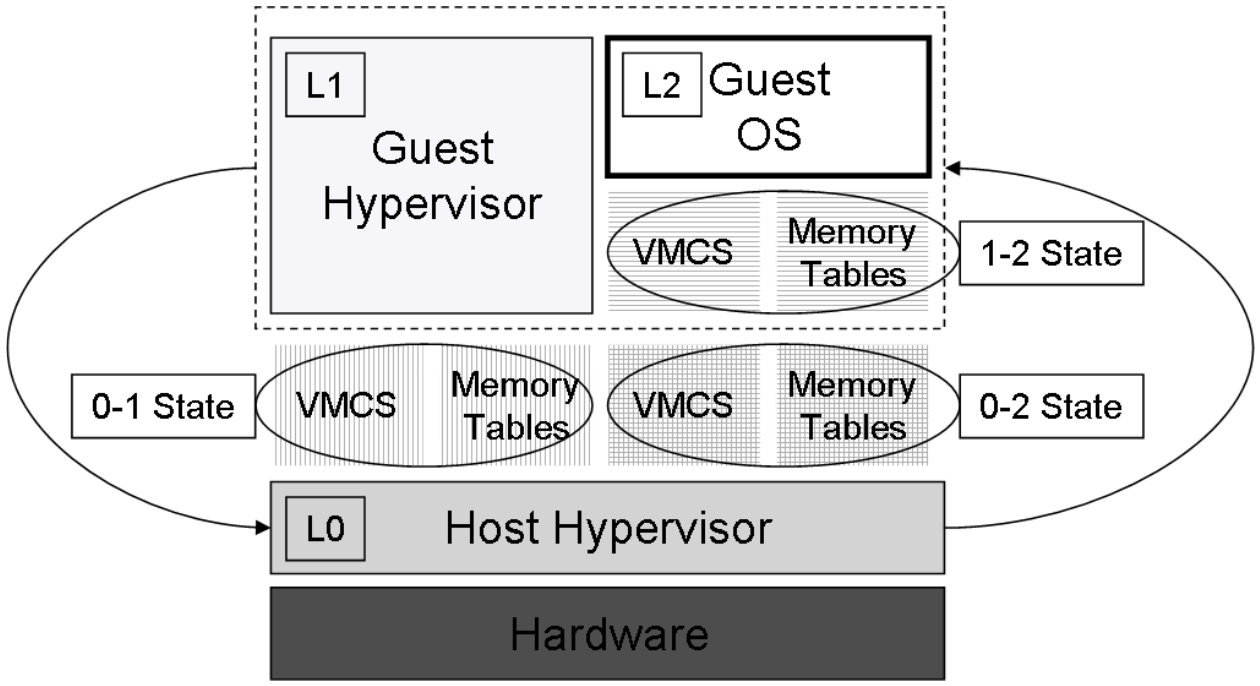
\includegraphics[width=0.82\linewidth]{figures/turtles-architecture.png}
\caption[嵌套虚拟化的总体架构]{嵌套虚拟化的总体架构：L1 与它管理的 L2 同处 L0 提供的一个虚拟机之内（虚线框），L0 为运行 L1 与运行 L2 各维护一份状态（0-1 与 0-2），L1 自己维护的 1-2 状态只存在于软件中。两侧弧形箭头表示 L0 与两台上层实体的运行关系：L0 借 0-1 状态运行 L1，借 0-2 状态运行 L2。引自 Ben-Yehuda et al., OSDI 2010, Figure 3~\cite{source7}。}
\label{fig:turtles-arch}
\end{figure}

图中三份状态都用 VMCS 与内存表（memory tables）两项表示，这正对应硬件虚拟化的两组对象：控制结构与地址翻译结构。0-1 是 L0 运行 L1 用的状态，0-2 是 L0 运行 L2 用的状态，二者都由 L0 维护并真正被硬件装载；1-2 是 L1 为 L2 准备的状态，图中以一个只存在于软件视角的方框表示——它从不进入处理器，只作为 L0 合成 0-2 的输入。同一张图也说明了嵌套的层级含义：硬件层之上只有 L0 一层 hypervisor 与它的虚拟机，L1 的“hypervisor 身份”完全由 L0 在软件中构造，这正是后面 CPU 与内存两节各自要展开的合成工作的出发点。

\subsubsection{CPU：虚拟化VMX与合成VMCS}\label{sec:nested-cpu}

在论文使用的单层 VMX 基线上，L1 在 VMX non-root 环境执行虚拟化管理指令会触发相应的拦截，这就给了 L0 一个天然的介入点：L0 捕获并模拟 L1 的 VMX 指令，也就是“trap-and-emulate”。大部分 VMX 指令的处理是“L1 退出到 L0、L0 按 VMCS 更新规则改写状态、再回到 L1”，让 L1 觉得指令真的执行了；但用来启动虚拟机的 \code{vmresume} 与 \code{vmlaunch} 是例外，因为此时 L0 必须模拟一次 L1→L2 的 VMEntry，流程变成“L1 退出到 L0，L0 直接 VMEntry 进入 L2”~\cite{source7}。

状态合成的关键是三份 VMCS 的分工，即图~\ref{fig:turtles-arch} 中三份状态各自的 VMCS 部分。VMCS01 是 L0 运行 L1 用的结构，从硬件角度看它和单层虚拟化完全一样：一个 hypervisor（L0）在 root mode 跑，一个 guest（L1）在 guest mode 跑。L1 为 L2 建立 VMCS12 来描述所需运行环境。该结构的地址与 host 状态具有 L1 视角下的含义，L0 不能不经检查、转换和合成就把它作为真实控制结构装载。于是 L0 以 VMCS12 为蓝本，再叠加 VMCS01 里对 L1 的约束，合成 VMCS02 作为真正运行 L2 的结构：guest state 大多可直接拷贝，host state 必须填成 L0 自己的、以便 CPU 从 L2 正确切回 L0，而 VMCS12 的 host state 要拷进 VMCS01 的 guest state，使 L0 模拟 L2→L1 切换时能加载正确的 L1 上下文~\cite{source7}。

控制数据的合成是正确性的重心。设想 L1 在 VMCS12 里要求 trap 某事件 $E_A$，但 L0 在 VMCS01 里并没有为 L1 trap 这个事件，那么为了把 $E_A$ 转发给 L1，L0 必须在 VMCS02 里补上对应的 trap；同理，L1 用来向 L2 注入事件的字段、以及 CPU 用来报告退出原因的字段都要合并。这套合并的具体实现落在 KVM 源码里，论文没有逐字段展开~\cite{source7}。这里有一个必须澄清的术语边界：Turtles 所说的 VMCS shadowing 是 L0 在软件层面“影子维护”VMCS12 并合成 VMCS02 的技术，与后来 Intel 在 Haswell 引入的同名硬件特性（让 L0 不必在每次 \code{vmread}/\code{vmwrite} 时都 trap）不是一回事；Turtles 的机制不依赖任何后续硬件能力~\cite{source7,source8}。同样，Turtles 描述的 2010 年合成逻辑，不应被当成当前 KVM 全部路径的写照——如今内核里的实现（如 \path{arch/x86/kvm/vmx/nested.c} 的 \code{prepare_vmcs02}）已经历多次重构并叠加了硬件加速，只可作为“合成 VMCS02 这一思路延续至今”的旁证，而非当年原型的源码~\cite{source5}。

\subsubsection{内存：EPT on top of EPT 的多维分页}\label{sec:nested-mem}

地址翻译在嵌套下多出一层：逻辑链是 L2 VA→L2 GPA→L1 GPA→host PA，即三层表。但当时的硬件 MMU 最多只支持两维（guest 页表 + EPT/NPT），无法同时走三层，因此必须把三层折叠到硬件提供的两层上。图~\ref{fig:turtles-mmu} 给出论文比较的三种折叠方式，区别在于哪一层由软件兜住：第一栏两层影子页表、第二栏影子页表叠在 EPT 上、第三栏才是 Turtles 采用的多维分页（图中标注为 EPT on top of EPT）。前两栏的共同点是 L1 用影子页表跑 L2，于是 L2 的每次页故障和每次页表写都要 L1 处理、并经 L0 转发；本节只展开第三栏，前两栏仅作为代价对照留在图上~\cite{source7}。

第三栏的关键是让两层都用 EPT 这一硬件结构，而不是让任何一层退化成影子页表。为此 L0 先向 L1 暴露 EPT 能力，使 L1 相信自己也能建 EPT，于是 L1 为 L2 建出 EPT12；但硬件只有一张 EPT，L0 不能直接装载 EPT12，便把它与自己的 EPT01 折叠成一张 EPT02。折叠的语义就是两次翻译的串接：L2 GPA 经 EPT12 得到 L1 GPA，再经 EPT01 得到 L0 的 host PA；EPT02 记录的是这条链的终点，因此硬件在实际执行时只需一次 EPT 遍历就完成 L2 GPA→host PA。图中第三栏下方那条从 L2 physical 直指 L0 physical 的 EPT02 箭头就是这个合成结果，而 EPT12 与 EPT01 两条箭头表示它由哪两段拼接而来；同时 L2 自己的页表（图中 GPT）仍然保留，负责 L2 VA→L2 GPA 这一层，硬件不替 L2 遍历它~\cite{source7}。

这张 EPT02 是按需建立的。L0 以一张空 EPT02 启动 L2，当 L2 访问的 GPA 在 EPT02 里缺项时触发 EPT violation 退出到 L0；L0 检查 L1 维护的 EPT12 是否已有该地址的合法映射——有，则把 EPT12 里的 L2→L1 映射与 EPT01 里的 L1→host 映射拼接后写入 EPT02 对应项；没有，说明这个缺页属于 L1 应负责的范围（例如 L1 尚未为该 GPA 分配内存），L0 就把退出交给 L1 处理，待 L1 更新 EPT12 后再回来补 EPT02~\cite{source7}。这个分流规则与 CPU 维度的退出归属判定同源：谁有权填这张表，缺项就归谁。

一致性维护是这套方案的固定开销。为保持 EPT02 与 EPT12 同步，L0 把 EPT12 所在内存设为只读，L1 一旦改写就 trap，L0 据此更新 EPT02 的相应项；L0 还要 trap L1 的 \code{INVEPT}，把 L1 意图的失效翻译成对自己 EPT 缓存的失效。两类 trap 的频率都由 EPT 表项数决定，因此 L0 允许用大页为 guest 内存做后备以缩小 EPT 表，也允许 L1 使用 VPID 给 TLB 条目打标签以免每次切换都冲刷 TLB；由于两侧都可自由选择 VPID 编号、可能冲突，L0 还需把 L1 自选的编号重映射到自己的有效编号~\cite{source7}。需要区分两类缺项：EPT02 缺项归 L0 补，L2 自身的普通页故障通常仍由 L2 处理，除非上层配置了相应拦截~\cite{source7}。

\begin{figure}[htbp]
\centering
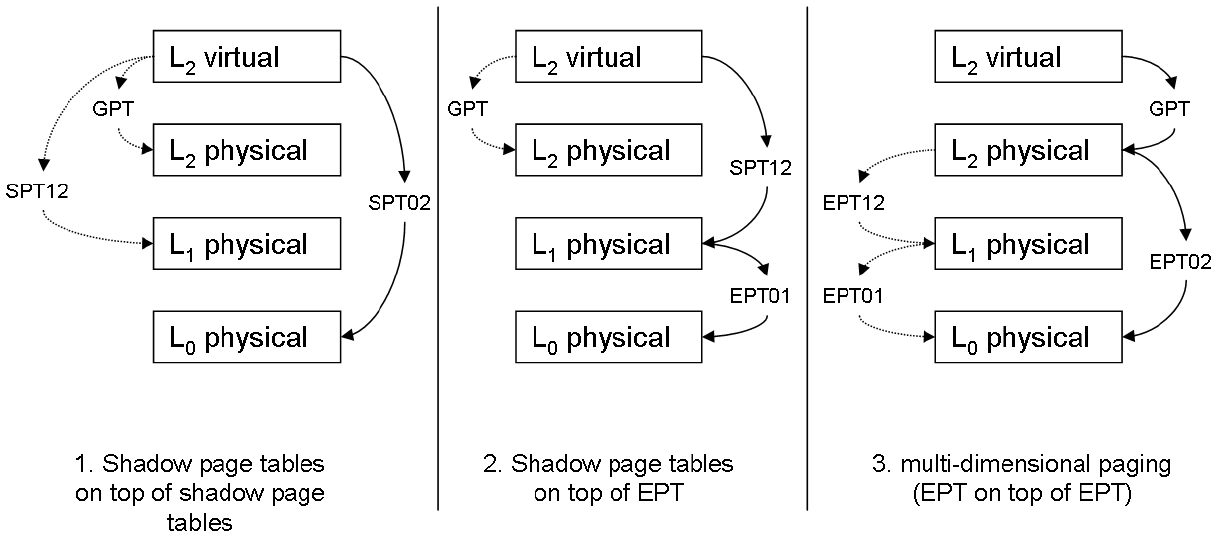
\includegraphics[width=0.98\linewidth]{figures/turtles-mmu-models.png}
\caption[三种嵌套 MMU 虚拟化模型]{三种嵌套 MMU 虚拟化模型：1. 影子页表叠在影子页表上；2. 影子页表叠在 EPT 上；3. 多维分页，即 EPT 叠在 EPT 上。四层方框自下而上为 L0 physical、L1 physical、L2 physical、L2 virtual，弧形箭头标注每段由哪张表承担（GPT、SPT12、SPT02、EPT01、EPT12、EPT02）。本文只展开第 3 栏。引自 Ben-Yehuda et al., OSDI 2010, Figure 4~\cite{source7}。}
\label{fig:turtles-mmu}
\end{figure}

\subsubsection{中断：事件归属、转发与注入}\label{sec:nested-irq}

嵌套下的中断必须分清三件不同的事：宿主自己产生的外部中断或 NMI，L0 要注入给 L1 的虚拟中断，以及 L1 希望注入给 L2 的事件。它们的处理路径不同。当 L2 正在运行且发生一次退出时，L0 首先按 VMCS12 与 VMCS02 的 trap 配置判断归属：属于 L0 的事件（外部中断、NMI，或只在 VMCS02 里 trap 的事件）就地处理后恢复 L2；属于 L1 的事件，L0 把 CPU 已更新的 VMCS02 字段拷回 VMCS12，再恢复 L1，让 L1 觉得是一次 L2→L1 的直接退出~\cite{source7}。注入方向上，L1 在 VMCS12 里写的注入字段要被 L0 合并进 VMCS02，才能让 CPU 真正把中断送进 L2。

设备分配场景揭示了一个关键的非对称性：DMA 直达不等于中断直达。多级设备分配让 L2 的数据可以直接落到设备，但中断在当时的 x86 架构上无法直接派发给 guest——中断到来总是先退出到 L0，L0 再转发 L1，L1 注入 L2，其中断的 EOI 写回也会再次触发退出。论文据此推断，设备中断及其 EOI 造成的退出是设备分配场景下残余开销的最大来源，并用一个去掉中断、纯轮询的网络驱动做了对照实验来支撑这一假设~\cite{source7}。需要强调的是，这是 2010 年原型在当时架构下的路径描述；后续硬件与 KVM 实现继续演进，因而不能把当年的中断处理路径断言为所有当前实现的必然行为~\cite{source7,source8}。

\subsubsection{设备：多级设备分配与虚拟IOMMU}\label{sec:nested-dev}

两层虚拟化各可选用模拟、半虚拟化或设备分配三种 I/O 方式，组合出九种可能，Turtles 重点评估了其中五种，并把“L0→L1 与 L1→L2 都做设备分配”称为多级设备分配~\cite{source7}。其目标不是把真实网卡“直通”给 L2 就完事，而是要在数据路径外补全三条辅助路径。

DMA 的地址问题是第一道坎：guest 驱动用的是 guest 物理地址，设备访存用的是 host 物理地址，而当时的 IOMMU 只支持一级翻译，两层映射必须再次压缩到一层。对可修改的 L1 可用半虚拟化 IOMMU——把 L1 里设置 L2→L1 映射的代码替换成对 L0 的 hypercall，L0 把映射里的 L1 地址换成对应 L0 地址后写入真实 IOMMU；对不改 L1 的方案，L0 为 L1 模拟一个 IOMMU，L1 以为自己在真 IOMMU 上建 L2→L1 映射，L0 截获这些映射、重映射 L1 地址、把 L2→host 的映射写到真实 IOMMU 上~\cite{source7}。中断路径如前所述仍需退出转发。MMIO 与 PIO 则相对干净：嵌套 guest 的 MMIO/PIO 与单层 guest 走同样的机制，不在 I/O 关键路径上引入额外退出~\cite{source7}。也就是说，多级设备分配的价值在于把 DMA 与 MMIO/PIO 留在直通路径上，代价集中在中断转发与 L1 注入这两类退出上，隔离和通知并没有被“直通”二字抹掉。

把四维放在一起看，Turtles 的“组合”有统一的形状：L1 表达的要求（VMCS12、EPT12、L1 侧的 IOMMU 映射）是输入，L0 自身的约束（VMCS01、EPT01、真实 IOMMU 的能力）是另一组输入，两者合并成一份硬件当下可执行的产物（VMCS02、EPT02、真实 IOMMU 里的映射表），而合并的依据始终是归属判定——退出归谁处理、缺项归谁填、设备地址归谁分配。图~\ref{fig:turtles-arch} 给出这一形状在整机层面的样子：三份状态中只有两份被硬件装载，第三份停留在软件里充当输入。

\subsection{Turtles 的开销与评测}\label{sec:turtles-cost}

Turtles 的成就是正确性与可行性：在不修改 guest hypervisor 的前提下给出了嵌套语义。但它的开销分析也暴露了问题的下一层形态。论文用 L2 里循环执行 \code{cpuid} 的合成微基准测单次退出的周期成本：裸机上 \code{cpuid} 约 100 周期，单层虚拟化约 2600 周期（其中约 1000 周期是模式切换），嵌套则飙到约 58000 周期~\cite{source7}。原因是 L1 每处理一次 L2 退出，都要执行多条 \code{vmread}/\code{vmwrite} 这类特权指令，而每条又各自触发一次对 L0 的退出——退出被逐级放大。论文在这里区分两类优化。L0 的合并路径可以只拷贝变化字段，并探索直接批量访问真实 VMCS 的方式；后一尝试不严格符合 VMX 规范，不能保证跨处理器适用。另一个称为 DRW 的评测配置则明确修改 L1，使其直接读写 VMCS12，用来估计省去 L1 的 VMREAD/VMWRITE 拦截的潜在收益。这两类直接访问不能混称为只修改 L0 的同一个优化~\cite{source7}。

论文的宏观负载报告给出同一方向的证据：在 KVM 同时充当 L0 与 L1 并启用多维分页的配置下，相对单层 guest，kernbench 的运行时间增加 14.5\%，SPECjbb 分数下降约 7.8\%；改用修改 L1、使其直接读写 VMCS12 的 DRW 配置后，两项数值分别变为 10.3\% 与 6.3\%~\cite[\S4.1, Table 2]{source7}。这些是论文报告值，不是本文复现。数值差异说明管理路径的密集程度会影响嵌套成本，摘要中的较低开销不能解释为适用于全部工作负载的上界；DRW 改动了 guest hypervisor，必须与未修改 guest 的基线分别讨论。

\subsection{小结：正确性之后剩下的成本}\label{sec:turtles-summary}

至此可以把 Turtles 的结论压成两句。正确性一侧，它把三层语义压进单层硬件支持：VMX 指令被 trap-and-emulate，VMCS12 作为需求说明书由 L0 合成为 VMCS02，EPT12 与 EPT01 折叠成 EPT02，L2 的 DMA 经虚拟或半虚拟 IOMMU 落到真实 IOMMU，而每一次退出由 L0 判定归属——属于它的事件就地处理后直接恢复 L2，属于 L1 的事件才转发。代价一侧，任何需要 L1 处理的退出都要走 $L2 \to L0 \to L1 \to L0 \to L2$，而 L1 处理时执行的 \code{vmread}/\code{vmwrite} 各自又触发一次对 L0 的退出，退出被逐级放大。两个边界需要重申：本章描述的是 2010 年原型在缺少嵌套架构支持时的实现，不能当作当前 KVM 全部路径的写照；DRW 这类配置改动了 guest hypervisor，其数字不能与未修改 guest 的结果混用。硬件后来加入的 VMCS shadowing 一类辅助改变的是复用的成本，而不是复用的必要性。成本究竟落在哪一段路径上、又该如何削减，是下一章的问题。

\section{嵌套虚拟化（二）：HyperTurtle 与跨层往返的削减}\label{sec:hyperturtle}

计算机领域有一句话：一件事如果复杂到不好直接描述，就不妨在中间加一层抽象。虚拟化本身就是这句话的产物——VMM 把整台机器的指令集、地址空间、中断与设备重新表述成一组虚拟接口，于是“在一台机器上跑多台机器”不再需要逐条处理每个细节，而变成对这套接口的一次实现。嵌套虚拟化是把同一层抽象再叠一次：L1 拿到的不是真实机器，而是一套虚拟的虚拟化接口，它用这套接口去管理 L2。

抽象层不是免费的。每穿过一次接口边界都要付出模式切换、状态翻译与事件转发的代价，叠了两层，这条路径就要走两遍。跨抽象层的性能优化由此成为一个独立的问题：目标不是取消抽象——那会连带丢掉隔离与管理权——而是让一部分操作不必真的穿过它，在保持接口语义的前提下把执行留在更靠底的那一层。HyperTurtle 正落在这个位置上：L1 hypervisor 通过 eBPF 把自身的处理逻辑注册成 L0 事件处理路径上的 hook，L2 触发相应事件时由 L0 就地调用这段程序完成处理，省掉进入 L1 的那次往返，而策略仍由 L1 定义~\cite{source8}。

上一章已经用普通嵌套的九步路径说明：当 $EPT_{0\to2}$ 与 $EPT_{1\to2}$ 都缺项时，L0 要先进入 L1 补蓝本，再让 L2 重执行、再次退出，最后才能补硬件实际使用的影子表。本章不再并列展开网络、采样和 artifact 程序，而是只沿这一次 $EPT_{0\to2}$ page fault 往下走：先分清两张 EPT 各自缺什么，再看 hyperupcall 如何借助 L1 中 QEMU 的页表和预分配帧池补 $EPT_{1\to2}$，最后分析 L0 如何收尾、L1 如何同步，以及何时必须回退。

图~\ref{fig:ht-worldswitch} 给出这一改法的总览：左栏普通嵌套把 L2 的事件经 L0 转发给 L1 hypervisor，右栏则由 L0 在处理路径上直接执行 hyperupcall。它强调的是处理位置的变化；本章随后补全图中略去的两张 EPT、QEMU 页表与回退条件。

\begin{figure}[htbp]
\centering
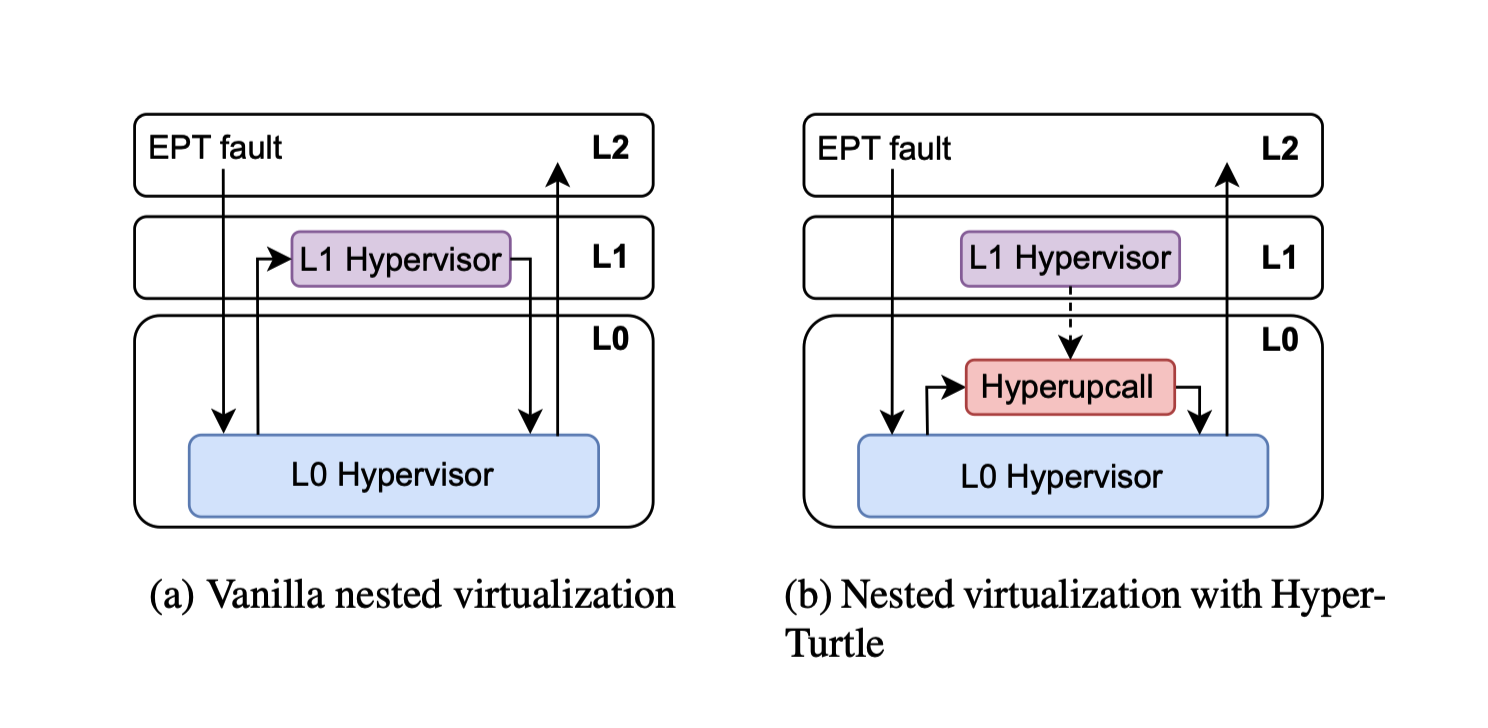
\includegraphics[width=0.98\linewidth]{figures/hyperturtle-fig1.png}
\caption[嵌套虚拟化中的 world-switch 问题]{嵌套虚拟化中的 world-switch 问题。(a) 普通嵌套：L2 的 EPT fault 由 L1 hypervisor 处理，L0 转发该事件并增加跨层切换；(b) HyperTurtle：L0 通过 hyperupcall 就地执行下放的 eBPF 处理逻辑。引自 Ben Zur et al., USENIX ATC 2025, Figure 1~\cite{source8}。}
\label{fig:ht-worldswitch}
\end{figure}

\subsection{从两张 EPT 缺项定位问题}\label{sec:ht-motiv}

L2 中的一次普通访存先由 L2 页表把 L2 虚拟地址翻译成 L2 物理地址（L2-PA），再由硬件当前装载的 $EPT_{0\to2}$ 把 L2-PA 翻译成 L0 物理地址（L0-PA）。后一跳缺项会触发 EPT violation，CPU 从 L2 退出到 L0，原访存指令尚未完成。L0 此时面对的不是一个孤立的“缺页”请求，而是两个必须分别回答的问题：L1 是否已经为这段 L2 内存分配了 L1 物理帧，以及 L0 是否已经把这个结果拼进 $EPT_{0\to2}$。

为区分这两件事，记发生 fault 的 L2-PA 为 $P$，承载它的 L1 物理帧地址为 $M$，最终机器物理地址为 $H$。两张表与 L0 自有的 $EPT_{0\to1}$ 形成如下关系：

\begin{equation}
EPT_{1\to2}:P\rightarrow M,\qquad
EPT_{0\to1}:M\rightarrow H,\qquad
EPT_{0\to2}:P\rightarrow H.
\end{equation}

其中 $EPT_{1\to2}$ 是 L1 KVM 为 L2 维护的蓝本，$EPT_{0\to1}$ 描述 L1 自身内存到真实机器内存的映射，$EPT_{0\to2}$ 则是 L0 为运行 L2 而合成的影子表。HyperTurtle 的 hook 不在每次 $EPT_{0\to2}$ 缺项时都接管，而是放在 L0 检查蓝本之后：只有 $EPT_{1\to2}$ 也为 non-present 时，才需要替代原本进入 L1 的那一段处理~\cite{source8}。

\begin{lstlisting}[style=pseudopy,caption={L0 对一次 L2 EPT fault 的缺项分流（逻辑伪代码）},label={lst:ht-dispatch}]
def handle_l2_ept_fault(P, access_type):
    # CPU 已从 L2 退出；P 是 L2-PA，指令尚未完成
    if ept12_lookup(P).present:
        # L1 已分配 L1 帧，L0 只需合成影子表项
        install_ept02_from_ept12(P)
        resume_l2()
        return

    # EPT12 也缺项：传统路径在这里把 fault 注入 L1
    if hyperupcall_ept_fault(P, access_type) == SUCCESS:
        install_ept02_from_ept12(P)  # hyperupcall 已补好蓝本
        resume_l2()                  # 不进入 L1
    else:
        inject_ept_fault_to_l1(P, access_type)
        resume_l1()                  # 保留原有慢路径
\end{lstlisting}

代码块~\ref{lst:ht-dispatch} 的第一条分支说明，$EPT_{0\to2}$ 缺项本身不等于 hyperupcall 必须工作；蓝本已有映射时，L0 直接补影子表即可。后一条分支才是本章的主线：hyperupcall 的任务是补 $EPT_{1\to2}$，不是替 L0 直接写 $EPT_{0\to2}$。它返回成功后，L0 仍按原有规则完成 $P\rightarrow M\rightarrow H$ 的合成，再恢复 L2。

普通嵌套下，这个“蓝本也缺”的情形造成六次 world-switch：L2 首次退出、L0 进入 L1、L1 恢复动作陷入 L0、L0 进入 L2、L2 重执行后再次退出、L0 最终恢复 L2。HyperTurtle 成功时把路径压成 $L2\rightarrow L0\rightarrow L2$：省掉的是进入 L1 建蓝本、L1 的恢复尝试，以及 L2 第一次重执行后的第二次 fault；L0 对影子表的建立并未被取消~\cite{source8}。

\subsection{hyperupcall 的注册与状态准备}\label{sec:hyperturtle-design}

HyperTurtle 把 L1 定义的这段建表逻辑写成 eBPF 程序，称为 hyperupcall。安装与执行必须分开理解：安装时，L1 通过 hypercall 把编译后的程序交给 L0，经 L0 的 KVM 与用户态安装组件完成验证和加载，再把程序链接到 L0 的 EPT fault hook。加载与链接拆成两个 hypercall，使同一程序可以挂到多个 hook 而不必重复加载。完成安装后，程序不再经 hypercall 调用，而是由 L0 在处理 L2 事件时直接触发~\cite{source8}。

这段程序不能任意读写 L1。新增 helper \code{bpf_probe_read_hyperupcall} 只允许它读取有效、已映射且属于其所属 L1 的物理内存；eBPF verifier 检查程序自身的内存访问、循环等约束，VM 归属与 helper 的地址检查再限定它能看哪一份 guest 状态。L0 与 L1 之间还通过共享的数组型 eBPF map 交换数据，map 经共享内存 PCI 设备映射到 L1，因而双方可以并发访问同一份状态，而不是每次借 VM-exit 传递消息~\cite{source8}。

EPT 案例需要预先准备四类共享状态：L1 维护的预分配帧池、QEMU 进程的页表根 \code{cr3}、记录 hyperupcall 所建映射的 fault log，以及记录 L1 侧 shmem 缺页的 page fault log；另有一把双方都能获取的共享锁。eBPF 上下文不适合完成复杂的内存分配，所以帧池由 L1 异步补充，或在其因 VM-exit 获得处理机会时批量补充。论文实验采用 4096 帧的池，以避免同步补充；池空不是错误，而是回退条件~\cite{source8}。

\subsection{沿一次 EPT fault 展开 HyperTurtle}\label{sec:nested-ht-ept}

本例采用论文限定的 shmem 文件后备内存：L1 中的 QEMU 通过 \code{mmap} 获得一段自己的虚拟内存，再把它注册为 L2 的 guest RAM。为叙述具体，以下直接称这一 VMM 为 QEMU；Cloud Hypervisor 在该路径中承担相同角色。论文原型面向 QEMU、Cloud Hypervisor 与 Kata Containers 所采用的这类后备方式，不能把结论直接推广到任意内存后端~\cite{source8}。

\subsubsection{先分清 QEMU 页表与 EPT}\label{sec:ht-qemu-pagetable}

QEMU 虽然管理 L2，本身仍是 L1 中的一个用户态进程。它访问自己的代码、堆和所映射的 L2 内存时，使用 L1 内核为其维护的普通进程页表：

\begin{equation}
\text{QEMU 的 L1-VA }V
\xrightarrow{\text{QEMU 页表}}\text{L1-PA }M.
\end{equation}

这里的“QEMU 页表”就是前面所说的 VMM 页表，不是 EPT，也不是 L2 中某个进程的页表。其根地址保存在 QEMU 进程的 \code{cr3} 中。QEMU 把一段起始虚拟地址为 $V_{\text{base}}$ 的内存注册成起始 L2-PA 为 $P_{\text{base}}$ 的内存槽后，同一页便有两个不同的名字：L2 看到 $P$，QEMU 看到 $V$。二者数值不必相等，逻辑位置由下式对应：

\begin{equation}
V=V_{\text{base}}+(P-P_{\text{base}}).
\end{equation}

QEMU 页表负责 $V\rightarrow M$，$EPT_{1\to2}$ 负责 $P\rightarrow M$。两棵树的根指针、输入地址空间和维护者都不同，不存在一方包含另一方的关系；它们只是可以在输出端指向同一个 L1 物理帧。L2 运行时使用 EPT，QEMU 自己访问该页时使用普通页表。HyperTurtle 读取 QEMU 页表，正是为了检查这页是否已经有一个可复用的 $M$。

\subsubsection{在 L0 内补全 L1 的蓝本}\label{sec:ht-upcall-body}

现在回到代码块~\ref{lst:ht-dispatch} 中调用 hyperupcall 的路径。L0 发现 $EPT_{1\to2}[P]$ 为 non-present 后，调用 hyperupcall，并传入 $P$ 与读写类型。程序首先尝试获取共享锁；成功后才检查 QEMU 页表、并发日志和帧池。整个快路径可概括为代码块~\ref{lst:ht-ept-body}。

\begin{lstlisting}[style=pseudopy,caption={hyperupcall 为缺失的蓝本寻找 L1 物理帧（逻辑伪代码）},label={lst:ht-ept-body}]
def hyperupcall_ept_fault(P, access_type):
    if not try_lock(shared_ept_lock):
        return FALLBACK
    if hyperupcall_fault_log.is_full():
        unlock(shared_ept_lock)
        return FALLBACK

    # 由内存槽的位置对应，算出 QEMU 看到的虚拟地址
    V = qemu_userspace_base(P) + (P - qemu_guest_phys_base(P))

    # 路径一：QEMU 已有 V -> M，复用这页，不再分配帧
    M = walk_qemu_page_table(shared_qemu_cr3, V)
    if M is not None:
        ept12_install(P, M, access_type)
        hyperupcall_fault_log.append(P)
        unlock(shared_ept_lock)
        return SUCCESS

    # QEMU 页表也没有：先看 L1 侧是否正在处理同一页
    if page_fault_log.contains(P):
        unlock(shared_ept_lock)
        return FALLBACK

    # 路径二：消费 L1 预分配的帧，补 EPT12 并通知 L1
    M = frame_pool.pop()
    if M is None:
        unlock(shared_ept_lock)
        return FALLBACK

    ept12_install(P, M, access_type)
    hyperupcall_fault_log.append(P)
    unlock(shared_ept_lock)
    return SUCCESS
\end{lstlisting}

遍历 QEMU 页表时，hyperupcall 并不把 QEMU 的 \code{cr3} 装入当前 CPU，也不切换到 QEMU 地址空间。它只是把共享的 \code{cr3} 当作页表根指针，使用受限 helper 逐级读取 QEMU 的普通页表项。若查到 $V\rightarrow M$，说明 QEMU 已经为这页建立好 L1 侧映射，程序可以直接构造 $EPT_{1\to2}:P\rightarrow M$，无需消耗帧池。

若 QEMU 页表也缺项，程序还不能立即分配，因为 L1 的 shmem 缺页路径或 \code{virtiofsd} 可能正在处理同一页。page fault log 用来暴露这类并发活动；若其中已有 $P$，hyperupcall 放弃快路径，由 L1 沿原有逻辑完成处理。只有没有并发冲突时，程序才从帧池取出 $M$，写入 $EPT_{1\to2}$，并把 $P$ 追加到 hyperupcall fault log。帧池耗尽、日志写满、取锁失败或遇到不支持的情况，都返回回退而不是在 L0 中勉强完成~\cite{source8}。

无论映射来自 QEMU 页表还是帧池，hyperupcall 返回成功时改变的都只是蓝本及共享日志。随后 L0 重新取得 $P\rightarrow M$，经 $EPT_{0\to1}$ 得到 $M\rightarrow H$，建立 $EPT_{0\to2}:P\rightarrow H$，恢复 L2。L2 重执行原访存指令，这一次第二级翻译已经齐全，不再需要为同一缺项第二次退出。

\subsubsection{恢复 L2 之后，L1 仍须同步}\label{sec:ht-ept-sync}

快路径结束于 L2，并不意味着 L1 的所有状态已经同步。尤其是从帧池取页时，$EPT_{1\to2}$ 已有 $P\rightarrow M$，QEMU 页表却可能仍没有对应的 $V\rightarrow M$。若让这种状态无限期滞留，QEMU 与其他共享该文件后备内存的组件就可能看到不一致的映射。HyperTurtle 因而把“让 L2 立即继续运行”与“把变化补记到 L1”拆成两个阶段。

代码块~\ref{lst:ht-ept-sync} 的两个函数有不同的触发者。第一个由 L1 KVM 在下一次因 VM-exit 进入 L1 时执行，用来消费 hyperupcall 留下的 fault log。第二个则是对 L1 原有 shmem page-fault handler 的包装：当 L1 中的 QEMU 或 \code{virtiofsd} 等文件后备内存使用者访问一个尚未在自身地址空间建立映射的 shmem 页，因而触发 L1 的普通页故障时，L1 内核进入这个包装函数。它不是 L2 发生 EPT fault 时由 L0 调用的 hyperupcall；前者处理 L1 进程地址空间的缺页，后者处理 L2 第二级地址翻译的缺项。

\begin{lstlisting}[style=pseudopy,caption={L1 后续补偿与 shmem 缺页路径的同步（逻辑伪代码）},label={lst:ht-ept-sync}]
def l1_on_next_vmexit():
    for P in hyperupcall_fault_log.drain():
        V = qemu_va_for_l2_pa(P)
        fault_qemu_va_into_address_space(V)  # 补 QEMU 页表等 L1 状态

def wrapped_l1_shmem_fault(P):
    spin_lock(shared_ept_lock)
    if ept12_lookup(P).present:
        map_existing_ept12_page_to_l1(P)  # hyperupcall 已先建映射
    original_shmem_fault_handler()
    page_fault_log.append(P)              # 告知 L0 侧程序：L1 处理过此页
    unlock(shared_ept_lock)
\end{lstlisting}

代码块~\ref{lst:ht-ept-sync} 的两个函数有不同触发者，此处分别说明。第一个由 L1 KVM 在下一次因 VM-exit 进入 L1 时执行，消费 hyperupcall fault log，并把其中 L2-PA 对应的 L1-VA fault 进 QEMU 地址空间。第二个则是对 L1 原有 shmem page-fault handler 的包装：当 L1 中的 QEMU 或 \code{virtiofsd} 等文件后备内存使用者访问一个尚未在自身地址空间建立映射的 shmem 页，因而触发 L1 的普通页故障时，L1 内核进入这个包装函数。它不是 L2 发生 EPT fault 时由 L0 调用的 hyperupcall；前者处理 L1 进程地址空间的缺页，后者处理 L2 第二级地址翻译的缺项。包装函数先取得同一把锁，再检查 $EPT_{1\to2}$ 是否已被 hyperupcall 填好；若已填好就复用该映射，随后执行原处理并记录 page fault log。这样，即使尚未发生一次进入 L1 的退出，L1 侧也不会忽略 L0 已经建立的映射~\cite{source8}。

这组机制也限定了 HyperTurtle 的实际贡献。它不是把 L1 从内存管理中删除，而是把 L2 继续运行所必需的蓝本建立留在 L0，把 L1 可见状态的补偿经日志延后；锁与双日志承担并发一致性，帧池承担资源供给，原 L1 路径承担所有快路径不适用的情况。优化的核心不是“eBPF 本身更快”，而是把一次跨层操作改造成一个有共享状态协议的就地处理路径。

\subsection{实验证据与适用边界}\label{sec:ht-eval}

上述机制的收益应当用同一条 EPT 路径衡量，而不能把不同子系统的加速比合并成“系统加速”。论文在 Kata 虚拟机内触发 1\,GiB 内存的按需映射，报告 HyperTurtle 相对普通嵌套 L2 的 EPT fault 平均延迟改善约 $5.25\times$、99p 延迟改善约 $4.76\times$；平均延迟接近其非嵌套参考，99p 则仍有约 8\% 差距~\cite[\S5.1]{source8}。这些数字支持的是“适用缺页热路径的往返显著减少”，不是任意访存都获得同样加速。

端到端意义来自 Kata 服务启动实验：论文从发出启动命令计时至容器内 Web 服务能够响应请求，而非只测 guest 内核 boot。不同镜像下，4\,KiB 页配置的平均启动时间缩短 27\%，2\,MiB 页配置为 8\%。大页情形仍有部分路径以 4\,KiB 页映射 L2 内核，因此优化并未完全失去作用，但收益较小~\cite[\S5.2]{source8}。这组结果说明收益依赖缺页在负载中的占比、页大小与后备内存组织；对已经建立好映射的稳定运行阶段，不能由启动结果外推同样的提升。

实验平台与配置也构成结论边界。论文使用双路 Xeon Silver 4216，固定 vCPU 与 vhost 线程在同一 NUMA 节点内的不同物理核，关闭 SMT，并设置 \codeplain{idle=poll} 与 \codeplain{nopti}。这些条件会影响空闲等待与隔离成本，因此本文只把数值视为论文报告，不将其当作生产环境的预先保证~\cite[\S5, Table 6]{source8}。

原型本身的限制更直接：EPT hyperupcall 不支持分配大页，对尚未映射进 QEMU 页表的部分 page-cache 页面不能直接处理，且全局 EPT hook 暂时只允许一个 L1 为一个 L2 使用该处理器。复杂 L1 功能的并发同步也限制了完整下放，所以原有 L1 路径必须长期保留~\cite[\S4.8]{source8}。后续评测若只继续降低理想路径延迟，仍不足以回答其可部署性；还应控制帧池补充频率、日志占用率和锁竞争，报告回退率、尾延迟及宿主 CPU 时间，检验省下的切换是否被一致性维护重新消耗。

安全边界同样需要与性能分开评价。verifier 约束的是程序执行形态，helper 的地址授权、VM 归属检查、日志协议与锁才决定它实际能访问和修改什么。该机制假定 L0 能读取并处理 L1 的相关状态，不能直接套用到把 L0 排除出信任边界的机密虚拟机模型。沿着本例可以得到一个更准确的总结：HyperTurtle 没有消除 $EPT_{0\to2}$ fault，也没有取代 L1 的内存管理；它把两张表都缺项时原本必须进入 L1 的一段工作，改为 L0 内可验证、可回退且带事后同步的处理，从而保留多层语义而缩短其关键路径。

\chapter*{结语}\phantomsection\addcontentsline{toc}{section}{结语}

回到本文开头的问题：怎样让客户机拥有一台机器的使用接口，却不拥有对真实资源的最终控制权。三种实现路径给出的答案并不构成一条简单的替代链，它们是同一问题在不同约束下的三种实现；其中嵌套一并两章，因为“把多层语义压到单层硬件上”与“削减由此产生的跨层往返”是两个先后相接、判据不同的问题。沿四维框架收束，可以得出三点判断。

第一，四个维度必须协作，任何单一维度都无法独立构成一台可用的虚拟机。CPU、内存、中断、设备各自解决执行、地址、异步事件与数据通路，而这些状态必须相互一致：地址转换的结果决定了访存与DMA是否落到正确的内存，中断投递要依赖CPU的执行上下文与设备的后端状态，设备完成通知又回到中断。软件方案里四者靠同一个进程内的数据结构连接，硬件方案里它们靠同一套异常级与系统结构的分工连接，嵌套方案里它们靠同一组跨层映射与事件归属连接\cite{source3,source4,source7}。割裂地看任何一个维度，都看不到整台机器为何能够运行。

第二，硬件辅助减少的是高频路径上的软件介入，管理策略与设备语义仍然需要软件。Stage-2把地址翻译下放给硬件，但内存后备的分配与映射维护仍是KVM的工作；在相应配置下，GICv4能向驻留vPE直接注入vLPI；映射配置、调度和doorbell响应仍需软件参与；SMMU约束真实DMA，却不能替代设备模型去实现网卡或磁盘的功能\cite{source4,source9,source10}。硬件提供的是机制，把机制组合成服务并决定何时使用它，仍是软件的责任。

第三，嵌套虚拟化的本质是把资源边界与上层策略组合起来，而这一步分成两个问题。Turtles 展示了将多层语义组合到现有硬件支持上的实现：VMX 指令由 L0 代执行、VMCS02 由两份配置合成、多层地址翻译折叠进一张 EPT，代价则集中在跨层往返与 L1 处理时的逐级放大~\cite{source7}。HyperTurtle 接着回答第二问，其适用范围是被安全下放且一致性成本可控的热路径——它依赖 verifier、受限 helper 与共享状态的同步协议维持相应隔离边界，并以回退路径兜底，因此优化的是适用的热路径，不取消 L1~\cite{source8}。两章合起来才构成完整判断：先把嵌套做对，再谈削减它的成本；前者的收益不能解释后者的加速比。

最后需要说明证据的边界。HyperTurtle的评测在固定绑核、关闭SMT、\codeplain{idle=poll}与\codeplain{nopti}的收紧配置下取得，网络吞吐实验还调整了vCPU数量，这些配置限定了实验中的资源争用、空闲等待和隔离开销条件\cite{source8}。因此论文报告的相对收益说明的是该配置下热路径优化的效果，不能直接外推为共享多租户生产环境的期望收益；本文未进行性能复现，对更广泛部署的适用性仍需通过独立实验检验。

把三种实现并置（嵌套两章合为一层来看），真正可比较的是执行、状态与策略被放在了哪里：软件把三者都放在进程内，硬件把机制下放而保留管理，嵌套则在资源边界与上层策略之间重新分配处理逻辑。虚拟化技术的演进，最终是在减少跨层操作与维持控制权之间不断寻找新的平衡点。

下表把三种方案在同一四维框架下并置，作为全文的收束。

\begin{table}[htbp]
\centering
\small
\begin{tabularx}{\linewidth}{@{}lYYY@{}}
\toprule
维度 & QEMU软件 & Arm硬件辅助 & x86-64嵌套 \\
\midrule
CPU & 翻译执行与软件CPU状态，guest指令由宿主代码实现 & guest在EL1/EL0原生执行，EL2控制，KVM切换上下文 & 虚拟化VMX与合成VMCS，按退出归属决定就地处理或转发 \\
内存 & 软件MMU与TLB，解释guest页表并映射到宿主内存 & Stage-1与Stage-2两阶段翻译，KVM管理Stage-2映射与相关异常 & 合成EPT压缩多层映射，维护映射一致性并下放部分缺页处理 \\
中断 & 软件控制器维护pending，经架构异常投递到guest & GICv3虚拟接口安排注入，GICv4对驻留vPE直接注入vLPI & 跨层事件转发与注入，减少特定处理路径的往返 \\
设备 & MMIO设备模型与软件DMA，后端完成请求并通知guest & 模拟、virtio与直通三种形态并存，SMMU约束真实DMA & 设备与IOMMU映射组合，下放数据处理与上层策略 \\
\bottomrule
\end{tabularx}
\caption{四维框架下的三种实现对照}
\label{tab:conclusion-dims}
\end{table}


\backmatter
\intotoc*{\cleardoublepage}{\bibname}
\bibliography{references}

\end{document}
